\documentclass[preprint,12pt]{elsarticle}

\usepackage{amsmath,amssymb,amsthm}
\usepackage[ruled,linesnumbered]{algorithm2e}
\theoremstyle{definition}
\newtheorem{proposition}{Proposition}
\newtheorem{definition}{Definition}
\usepackage{booktabs}
\usepackage{array}
\usepackage{threeparttable}
\usepackage{graphicx}
\usepackage{float}
\usepackage{hyperref}
\hypersetup{hidelinks}
\usepackage{setspace}
\usepackage[nopatch=footnote]{microtype}
\usepackage{pdflscape}
\usepackage{adjustbox}

\graphicspath{{ProvidedFigures/}{Charts/}}

\journal{}

\raggedbottom
\clubpenalty=10000
\widowpenalty=10000
\displaywidowpenalty=10000
\interfootnotelinepenalty=10000
\setlength{\emergencystretch}{2em}

% Float packing: let LaTeX place multiple figures per page instead of one-per-page.
\setcounter{topnumber}{3}
\setcounter{bottomnumber}{2}
\setcounter{totalnumber}{4}
\renewcommand{\topfraction}{0.94}
\renewcommand{\bottomfraction}{0.85}
\renewcommand{\textfraction}{0.06}
\renewcommand{\floatpagefraction}{0.72}

\makeatletter
\renewcommand{\footnoterule}{%
  \kern -3pt
  \hrule width .4\columnwidth
  \kern 2.6pt
}
\makeatother


% --- supplement-specific ---
\usepackage{xr-hyper}
\externaldocument{paper}              % resolve \ref to the main paper's labels
\renewcommand{\thesection}{S\arabic{section}}
\renewcommand{\thesubsection}{S\arabic{section}.\arabic{subsection}}
\renewcommand{\thetable}{S\arabic{table}}
\renewcommand{\thefigure}{S\arabic{figure}}
\renewcommand{\theproposition}{S\arabic{proposition}}

\begin{document}

\begin{frontmatter}
\title{Supplementary Appendix to\\ ``Structure-Preserving Randomization Inference for Decision Timing''}
\author{Aryan Patel}
\begin{abstract}
\noindent This appendix collects the implementation details, the full validation
suite, the additional empirical analyses, and the reproducibility material that
support the main paper. Section and equation references of the form ``Section~4''
or ``Proposition~1'' point to the main paper; references prefixed ``S'' are internal
to this appendix. Every reported quantity is the direct output of the accompanying
code on the canonical data, and the reproduction commands are listed in
Section~\ref{supp:repro}.
\end{abstract}
\end{frontmatter}

\setcounter{section}{0}

\section{Implementation details}
\label{supp:implementation}

To begin, this section specifies the data pipeline, trade generation, Monte Carlo and robustness machinery, the execution and fill model, and the strategy rule set summarized in the main paper.

\subsection{Data preparation}

The market sample consists of auto-adjusted daily open, high, low, close, and volume observations. The raw series is cleaned before any strategy is evaluated. Duplicate timestamps are removed, observations with missing or non-positive prices are discarded, negative volume values are reset to zero, and no missing bars are imputed. We do not impute because imputation would create artificial prices, artificial holding periods, or artificial trades; this is a deliberate, conservative choice.

A common feature table is then constructed for all strategies. The feature set includes a 20-bar exponential moving average; 20-, 50-, 100-, and 200-bar simple moving averages; one-bar close-to-close returns; rolling return volatility; 20-bar average volume and volume ratios; RSI(14); ATR(14); ATR as a fraction of price; ADX(14) with positive and negative directional indicators; Bollinger Bands; MACD; lagged rolling highs and lows; trailing returns over multiple horizons; relative volatility ratios; and a 20-bar price $z$-score. Any rolling high or low used in a trading rule is shifted by one bar so that the signal observed at date $t$ depends only on information available by the close of date $t$.

Market regimes are assigned after feature construction. Here, \(\sigma_t\) is the 20-bar rolling standard deviation of close-to-close returns. For each date, the lower and upper regime thresholds are the one-third and two-third expanding quantiles of \(\{\sigma_u\}_{u<t}\), shifted by one bar so that the current label is forward-safe. We activate regimes only after 120 daily bars of history are available, because the expanding quantiles are unstable before then. Each bar is classified as \emph{calm}, \emph{neutral}, or \emph{stressed}. The expanding-quantile construction is forward-safe in the strict sense that the label at $t$ uses only information dated $\le t-1$; still, the cutoff levels themselves stabilize only as the expanding window grows, so early-sample labels are noisier than late-sample labels and are downweighted implicitly by the 120-bar warm-up.

\subsection{Trade generation}

All strategies are evaluated under a common execution model. Signals are formed on the completed bar at time \(t\), but entries occur at the next bar's open, \(t+1\), because a signal read off the close cannot be acted on until the market reopens. Exit conditions are also evaluated on completed bars and executed at the following open. We impose this next-bar execution rule uniformly across the entire strategy panel so that no strategy gains an advantage from same-bar fills.

Fills are adverse to the trader at the next-bar open and incorporate a half-spread, per-side slippage, and per-order commissions; positions do not overlap, and we reject a candidate entry when no exit bar remains, when the next open gaps through the intended stop or target, or when position size is infeasible under the capital and liquidity constraints. The full execution and fill model (initial capital, the liquidity cap, share rounding, the exact cost schedule, and the gap and overlap rules) is specified in \ref{app:execution}. These assumptions imply an expected round-trip cost of $c=0.000470$ in return units, which we apply identically to the realized strategy and to every simulated schedule, because the comparison is fair only when both sides face the same frictions.

The main text reports the strategy families rather than every threshold and stop rule. The panel contains trend-following, breakout, mean-reversion, volatility-filtered, calendar, and random-control rules. We fixed all thresholds before the reported GC=F run and do not re-optimize them inside the paper, because re-optimizing on the same data we test on would manufacture exactly the skill we are trying to detect. We place the full implementation definitions in \ref{app:strategy_rules} so that the empirical section can focus on the null construction and evidence.

Each completed position is stored in a standardized trade record containing the signal date, entry and exit timestamps, reference and executed prices, quantity, commissions, slippage, capital before and after the trade, deployed capital, portfolio weight, gross and net profit and loss, gross and net returns, portfolio-level return contribution, holding period, regime at entry, stop and target levels, and exit reason. Separate descriptive summaries record the number of candidate signals, the number of executed trades, rejected signals, and months covered.

\subsection{Monte Carlo simulation}

The null comparison is run separately for each strategy. We impose reproducibility through a fixed initial seed of 42, from which independent strategy-specific pseudo-random streams are derived; this means anyone re-running the code lands on the same null draws. The default simulation depth is
\begin{equation}
M=5{,}000
\end{equation}
draws per strategy.

The realized cumulative return is computed directly from the saved trade-level portfolio returns. Here, \(r_j\) is the portfolio return contribution of trade \(j\); then
\begin{equation}
CR_s^{\mathrm{actual}}
=
\exp\left(\sum_{j=1}^{N_s}\log(1+r_j)\right)-1.
\end{equation}
These realized trade returns are already net of execution costs. If a strategy generates no completed trades, we set the null distribution to a degenerate sequence of zero returns, because the downstream inference must remain well defined even when there is nothing to score.

Each randomized trade schedule is priced on the observed open-price calendar, with entry and exit reference prices given by the randomized opening prices at the simulated entry and exit indices. The simulation reapplies the same execution-cost and fill model used for the realized trades (\ref{app:execution}), because the realized strategy and its null comparison must face identical frictions; this implies the expected round-trip cost of $0.000470$. Here, \(\tilde{q}_{j,m}\) is the simulated net position return of trade \(j\) in simulation \(m\); the simulated portfolio return contribution is then
\begin{equation}
\tilde{r}_{j,m}=\omega_j \tilde{q}_{j,m},
\end{equation}
and the cumulative simulated return is
\begin{equation}
CR_{s,m}^{\mathrm{sim}}
=
\exp\left(\sum_{j=1}^{N_s}\log(1+\tilde{r}_{j,m})\right)-1.
\end{equation}

For each strategy, we retain the full simulated distribution together with a summary containing the realized cumulative return, the simulated mean, median, and standard deviation, the 5th and 95th simulated percentiles, the one-sided empirical \(p\)-value, the realized percentile rank, and the number of realized trades. We also adjust the one-sided \(p\)-values across the active strategy set using the Benjamini--Hochberg procedure, because several strategies are tested at once and the raw \(p\)-values would otherwise overstate significance.

\subsection{Robustness design}

We assess seed sensitivity through an outer robustness loop, because a single seed produces a single null draw and we want to know whether the verdict survives a change of seed. The default robustness configuration is
\begin{equation}
R=100, \qquad M_{\mathrm{rob}}=5{,}000,
\end{equation}
with outer-run seed
\begin{equation}
\text{seed}_r = 100 + r, \qquad r=1,\ldots,100.
\end{equation}
Each outer run again generates independent strategy-specific pseudo-random streams. For deterministic strategies, we hold the realized trade log fixed across outer runs and let only the null simulations vary, because the realized trades themselves do not depend on a seed. We treat the random baseline differently: under each outer-run seed, its realized trade sequence is regenerated before the null is evaluated, so both the realized outcome and the null distribution vary across runs. This means the random baseline carries seed noise on both sides, exactly as it should.

Each outer-run record stores the realized cumulative return, annualized return, annualized Sharpe ratio, trade-level return ratio, maximum drawdown, simulated mean, median, and standard deviation, the 5th and 95th null percentiles, the one-sided \(p\)-value, \(p\)-value prominence, percentile rank, \(\mathrm{RCSI}\), \(\mathrm{RCSI}_z\), and the number of trades. Annualized return is computed by annualizing the summed log trade returns over the active span from first entry to last exit using the observed bar density of the market calendar. Annualized Sharpe ratio and maximum drawdown are computed from a reconstructed bar-by-bar equity curve that marks open positions to market using close prices and carries idle periods in cash. The robustness summary then aggregates each metric across outer runs by its mean, median, standard deviation, minimum, maximum, and interquartile range, and reports the proportion of runs with \(p\le 0.05\) and the proportion of runs above the null median.

\subsection{Verdict classifier}

\paragraph{Verdict classifier.} The labels Strong / Moderate / Above-median / Random or luck / Below null median are deterministic functions of $(p, \pi, \mathrm{RCSI}_z)$, evaluated in order: \emph{Strong} if $\mathrm{RCSI}_z \ge 2.0$, $p\le 0.05$, and $\pi\ge 95$; \emph{Moderate} if $\mathrm{RCSI}_z\ge 1.0$, $p\le 0.05$, and $\pi\ge 85$; \emph{Above-median (not significant)} if $\mathrm{RCSI}_z\ge 0.5$, $p\le 0.20$, and $\pi\ge 70$; \emph{Random or luck} if $-0.5\le\mathrm{RCSI}_z\le 0.5$ and $0.30\le p\le 0.70$; and \emph{Below null median} if $\mathrm{RCSI}_z<-0.5$ and $p>0.50$; any case matching none of these defaults to Random or luck. We fix the thresholds ex ante, because optimizing them on the data would invite exactly the classifier-drift criticism we want to avoid; they are not optimized on the data. The three positive tiers require agreement of all three metrics, so the $p$-value and percentile (not the right-skewed $\mathrm{RCSI}_z$ in isolation) carry the inferential weight. In other words, a strategy ``below the null median'' is one whose realized return is worse than the null on both its tail probability and its standardized distance (here Trend Pullback and the Random baseline), which is a stricter condition than simply ranking below the median.

\subsection{Execution and fill model}
\label{app:execution}

Each strategy begins with \$100{,}000 of capital. The default maximum capital allocation per trade is $100\%$ of available capital, and the liquidity cap is $5\%$ of $20$-bar average volume. Non-crypto assets are traded in integer share quantities, while crypto assets are traded in increments of $0.0001$ units. Entry and exit fills are adverse to the trader: the reference price is the next-bar open, the half-spread is $0.5$ basis points, slippage on each side is drawn uniformly from $0.5$ to $3.0$ basis points, and the per-order commission for non-forex, non-crypto assets is $\max(0.005\times\text{shares},\,\$1)$. A candidate entry is rejected if no later bar remains for exit, if the next open gaps through the intended stop or target before the position is established, or if position size is infeasible after applying the capital and liquidity constraints. Positions do not overlap within a strategy; when both the stop-loss and take-profit are touched within the same bar, the stop-loss path is taken conservatively; and any surviving open position is liquidated at the last available open in the sample. The Monte Carlo null reprices each simulated schedule under this same model: a half-spread of $0.5$ basis points, a fresh per-side slippage draw on $[0.5,3.0]$ basis points, and an expected commission rate of $0.00002$, so that the realized strategy and its null comparison paths face identical frictions. Together these imply the expected round-trip cost $c=0.000470$ used throughout.

\subsection{Strategy rule definitions}
\label{app:strategy_rules}

The eleven reported strategies are implemented as follows.
\begin{itemize}
\item \textbf{Trend Pullback.} Entry requires the 50-bar moving average to exceed the 200-bar moving average, the close to exceed the 50-bar moving average, ADX to be at least 18, a pullback to or through the 20-bar exponential moving average, RSI(14) in the interval \([35,65]\), and a close at least as high as the previous close. The stop is the minimum of the current low and the lagged 10-bar low, less one ATR. The target is the lagged 20-bar high, with a fallback 2:1 reward-to-risk target if that level is not above the signal close. Exit occurs on stop, target, or failure of the long-horizon trend filter.

\item \textbf{Breakout Vol+Mom.} Entry requires either a close above the lagged 20-bar high or a near-breakout close within 0.2\% of that level, together with a participation filter, a momentum filter, and ADX of at least 18. Participation is defined by a volume ratio of at least 1.1 when volume is informative, or by a range-expansion condition of at least \(1.03\times\) ATR otherwise. Momentum is defined by MACD above its signal line or a 12-bar return of at least 0.5\%. The stop is the minimum of the current low and the lagged 10-bar low, less one ATR. The target is set at a 2:1 reward-to-risk multiple. Exit occurs on stop, target, failed breakout, or a 15-bar time stop.

\item \textbf{Mean Rev Vol Filter.} Entry requires a non-stressed, low-volatility, low-trend environment: ADX below 25, either the ATR ratio or the Bollinger-width ratio no greater than 1.6, and an absolute distance from the 50-bar moving average no greater than 3\%. The oversold trigger is the current low at or below the lower Bollinger band within a 0.2\% buffer, together with RSI(14) no greater than 35. The stop is the minimum of the current low and the lagged 5-bar low, less one ATR. The target is the Bollinger midpoint. Exit occurs on stop, target, reversion to the midpoint, or RSI recovery to at least 50.

\item \textbf{Validation AVM.} Entry requires the close above the 200-bar moving average, the 50-bar moving average at or above the 200-bar moving average, positive 20-bar and 60-bar returns, MACD above its signal line, ADX of at least 10, RSI(14) in \([45,82]\), an ATR ratio no greater than 1.9, a non-stressed regime, and either a reclaim of the 20-bar exponential moving average or a breakout above the lagged 20-bar high with volume confirmation. The stop is the lower of the lagged breakout low and the signal close minus \(2.2\times \mathrm{ATR}\). The target is the signal close plus \(6.0\times \mathrm{ATR}\). Position size is additionally scaled inversely with the ATR ratio, floored at 35\% and capped at 100\% of available capital. Exit occurs on stop, target, trailing stop, volatility shock, trend or momentum breakdown, or an 80-bar time stop.

\item \textbf{ADX Trend.} Entry requires the close above the 200-bar moving average, the 50-bar moving average at or above the 200-bar moving average, a positive 20-bar return, positive directional dominance, ADX of at least 18 and rising, an ATR ratio no greater than 2.2, and a non-stressed regime. The stop is the minimum of the lagged 10-bar low and the signal close minus \(2.0\times \mathrm{ATR}\). The target is the signal close plus \(4.0\times \mathrm{ATR}\). Exit occurs on stop, target, a reversal defined by the close below the 20-bar exponential moving average together with negative directional dominance, or a 90-bar time stop.

\item \textbf{Oversold Reversion.} Entry requires the close above the 200-bar moving average, the 50-bar moving average at or above the 200-bar moving average, a 20-bar price \(z\)-score no greater than \(-1.2\), either a touch of the lower Bollinger band or RSI(14) no greater than 40, a close at least as high as the previous close, and a non-stressed regime. The stop is the minimum of the current low and the signal close minus \(1.5\times \mathrm{ATR}\). The target is the signal close plus \(2.5\times \mathrm{ATR}\). Exit occurs on stop, target, recovery to the 20-bar exponential moving average, or a 20-bar time stop.

\item \textbf{Squeeze Breakout.} Entry requires volatility compression, defined by a Bollinger-width ratio no greater than 0.85, a breakout above the lagged 20-bar high, MACD above its signal line, ADX of at least 14, a volume ratio of at least 0.95 when volume is available, the close above the 200-bar moving average, and a non-stressed regime. The stop is the minimum of the lagged 10-bar low and the signal close minus \(1.8\times \mathrm{ATR}\). The target is the signal close plus \(3.5\times \mathrm{ATR}\). Exit occurs on stop, target, trailing stop, breakout failure, or a 45-bar time stop.

\item \textbf{Connors RSI2.} A Wilder-style RSI(2) and a 5-bar moving average are computed from closing prices. Entry requires the 50-bar moving average at or above the 200-bar moving average, the close above the 200-bar moving average, RSI(2) no greater than 5, a close no higher than the previous close, and a non-stressed regime. The stop is the minimum of the current low and the signal close minus \(1.5\times \mathrm{ATR}\). Exit occurs on stop, RSI(2) recovery to at least 70, recovery to the 5-bar moving average, break of the 200-bar trend filter, or an 8-bar time stop.

\item \textbf{Donchian Reentry.} Entry requires the close above the 200-bar moving average, the 50-bar moving average at or above the 200-bar moving average, a close above the lagged 55-bar Donchian high with no breakout on the previous bar, MACD at or above its signal line, ADX of at least 15, and a non-stressed regime. The stop is the minimum of the lagged 20-bar low and the signal close minus \(2.0\times \mathrm{ATR}\). The target is the signal close plus \(4.0\times \mathrm{ATR}\). Exit occurs on stop, target, loss of 50-bar trend support, momentum fade, or an 80-bar time stop.

\item \textbf{Turn-of-Month.} A signal is generated on the last trading day of each calendar month. Entry additionally requires a non-stressed regime and the close above the 200-bar moving average. The stop is the signal close minus \(2.0\times \mathrm{ATR}\). Exit occurs on stop, break of the trend filter, or completion of a fixed 4-bar holding window.

\item \textbf{Random.} This control strategy ignores market features. On each bar, entry occurs with probability 0.07, subject to the same feasibility, cost, sizing, and non-overlap rules as the rule-based strategies. At entry, the holding period is drawn uniformly from 4 to 18 bars, and exit occurs only when that planned holding period is reached. The main single-ticker run uses a fixed random seed of 42 for this baseline.
\end{itemize}

\section{Validation in known-truth environments}
\label{sec:supp-synthetic}

The previous sections define the null and its conditional interpretation. This section asks whether the procedure behaves sensibly when the data-generating environment is known, because a test must return the correct answer where the truth is known. The accompanying script \texttt{Code/synthetic\_timing\_experiments.py} constructs five synthetic worlds: IID no-skill returns, volatility clustering without entry skill, drift-only profitability, a high-exposure structural case whose profitability is intentionally absorbed by the conditioning set, and a deterministic entry-signal case. We evaluate each world with 1{,}500 replications and 2{,}000 null simulations per replication, and we report a Kolmogorov--Smirnov test of whether the no-skill $p$-values are uniform on $[0,1]$, because that uniformity is exactly what calibration requires. The power curve uses 400 replications per signal strength.

\begin{table}[H]
\centering
\caption{Synthetic validation summary ($1{,}500$ replications, $2{,}000$ null simulations each). Rejection rates are one-sided at $\alpha=0.05$ with the Monte Carlo standard error in parentheses; KS $p$ is the Kolmogorov--Smirnov test of $p$-value uniformity (large values are consistent with calibration).}
\label{tab:synthetic_validation}
{\small
\renewcommand{\arraystretch}{1.12}
\begin{adjustbox}{max width=\textwidth}
\begin{tabular}{@{}lrrrrrr@{}}
\toprule
World & Mean actual return & Mean $p$ & Reject @ 5\% (SE) & KS $p$ (unif.) & Profitable rate & Mean $\mathrm{RCSI}_z$ \\
\midrule
IID no skill & -0.004 & 0.506 & 0.051 (0.006) & 0.515 & 0.442 & -0.009 \\
Volatility clustering, no skill & \phantom{-}0.003 & 0.499 & 0.049 (0.006) & 0.701 & 0.469 & \phantom{-}0.009 \\
Drift only, no skill & \phantom{-}0.155 & 0.496 & 0.056 (0.006) & 0.598 & 0.767 & \phantom{-}0.018 \\
Structural exposure absorbed & \phantom{-}0.622 & 0.499 & 0.055 (0.006) & 0.566 & 0.929 & \phantom{-}0.007 \\
Entry signal & \phantom{-}2.044 & 0.001 & 1.000 (0.000) & $<0.001$ & 1.000 & \phantom{-}7.194 \\
\bottomrule
\end{tabular}
\end{adjustbox}
}
\par\vspace{0.5em}
\begin{minipage}{0.95\textwidth}
\centering
\footnotesize\emph{Notes.} The structural-exposure world uses a profitable long-exposure design with random entry placement. Its high profitable rate and nominal rejection rate illustrate the intended limitation of the test: profitable structure is not counted as entry-placement skill after conditioning on realized geometry. The entry-signal world samples an exogenous event schedule from $\mathbb{Q}$ and injects a positive return increment of 35 basis points per event bar at those selected windows; its low KS $p$ correctly reflects non-uniformity under the alternative.
\end{minipage}
\end{table}

The no-skill worlds are well calibrated. At $1{,}500$ replications the $\alpha=0.05$ rejection rate is $0.051$ for IID, $0.049$ for volatility clustering, $0.056$ for drift-only, and $0.055$ for the structural-exposure world; every one sits within about one Monte Carlo standard error ($\approx 0.006$) of nominal. The Kolmogorov--Smirnov test cannot reject uniformity of the no-skill $p$-values in any world (KS $p$ between $0.52$ and $0.70$), so the test is calibrated in distribution and not merely at the $5\%$ point. The structural-exposure case is the sharpest illustration of the intended estimand: it is profitable in $92.9\%$ of replications yet rejects at only $0.055$, because long exposure to a favorable path is conditioned away rather than counted as entry-placement skill. It is important to note that an earlier $200$-replication run had reported an IID rejection rate of $0.080$; at $1{,}500$ replications this resolves to $0.051$, which confirms it was Monte Carlo sampling noise rather than over-rejection.

\begin{figure}[htbp]
\centering
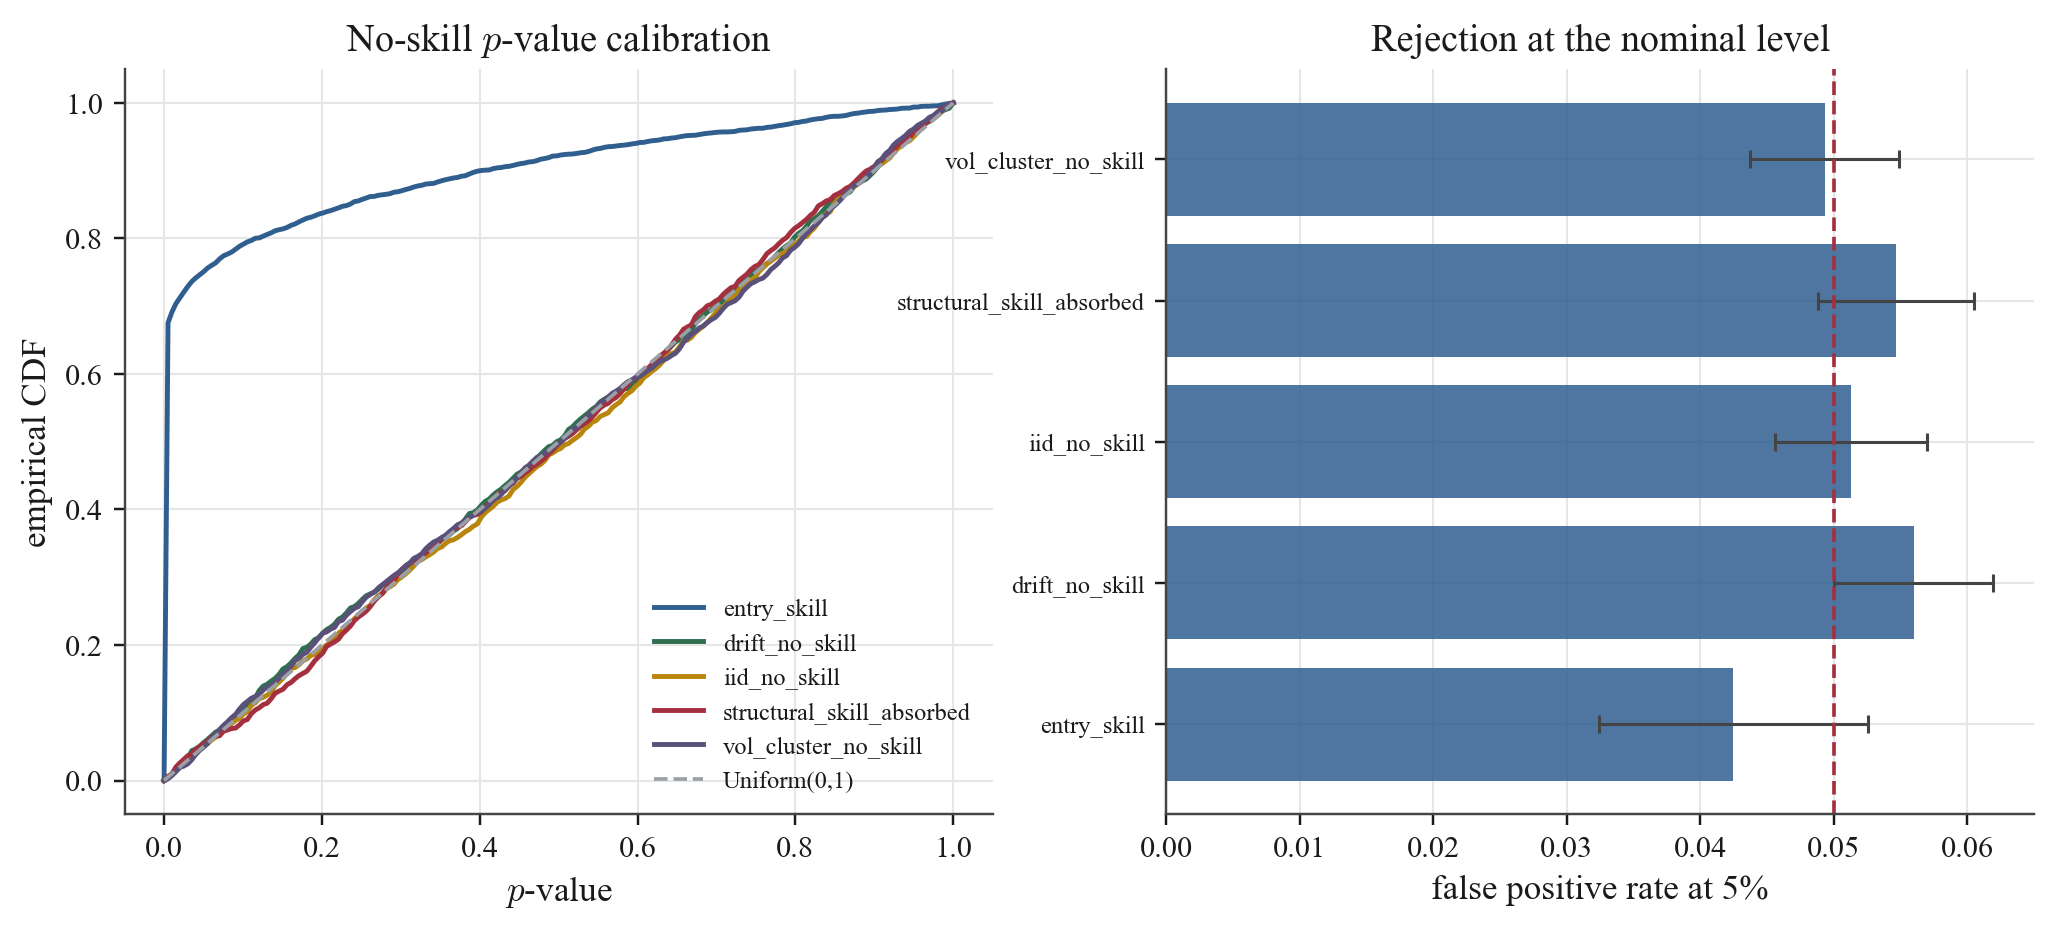
\includegraphics[width=0.95\textwidth]{synthetic_type1_calibration.png}
\caption{Synthetic p-value calibration under no-entry-skill worlds. The left panel compares empirical p-value CDFs with the uniform benchmark; the right panel reports false positive rates at the 5\% level.}
\label{fig:synthetic_calibration}
\end{figure}

Power rises monotonically with the injected entry signal. With no signal the 5\% rejection estimate is $0.043$ in the power-curve sample; at 5 basis points per event bar it rises to $0.130$, at 10 basis points to $0.475$, at 20 basis points to $0.925$, and at 35 basis points to $1.000$. The method detects sufficiently strong entry placement. Still, we are careful not to oversell it: weak signals and small trade counts can be underpowered, and we keep that warning in view throughout.

\begin{figure}[htbp]
\centering
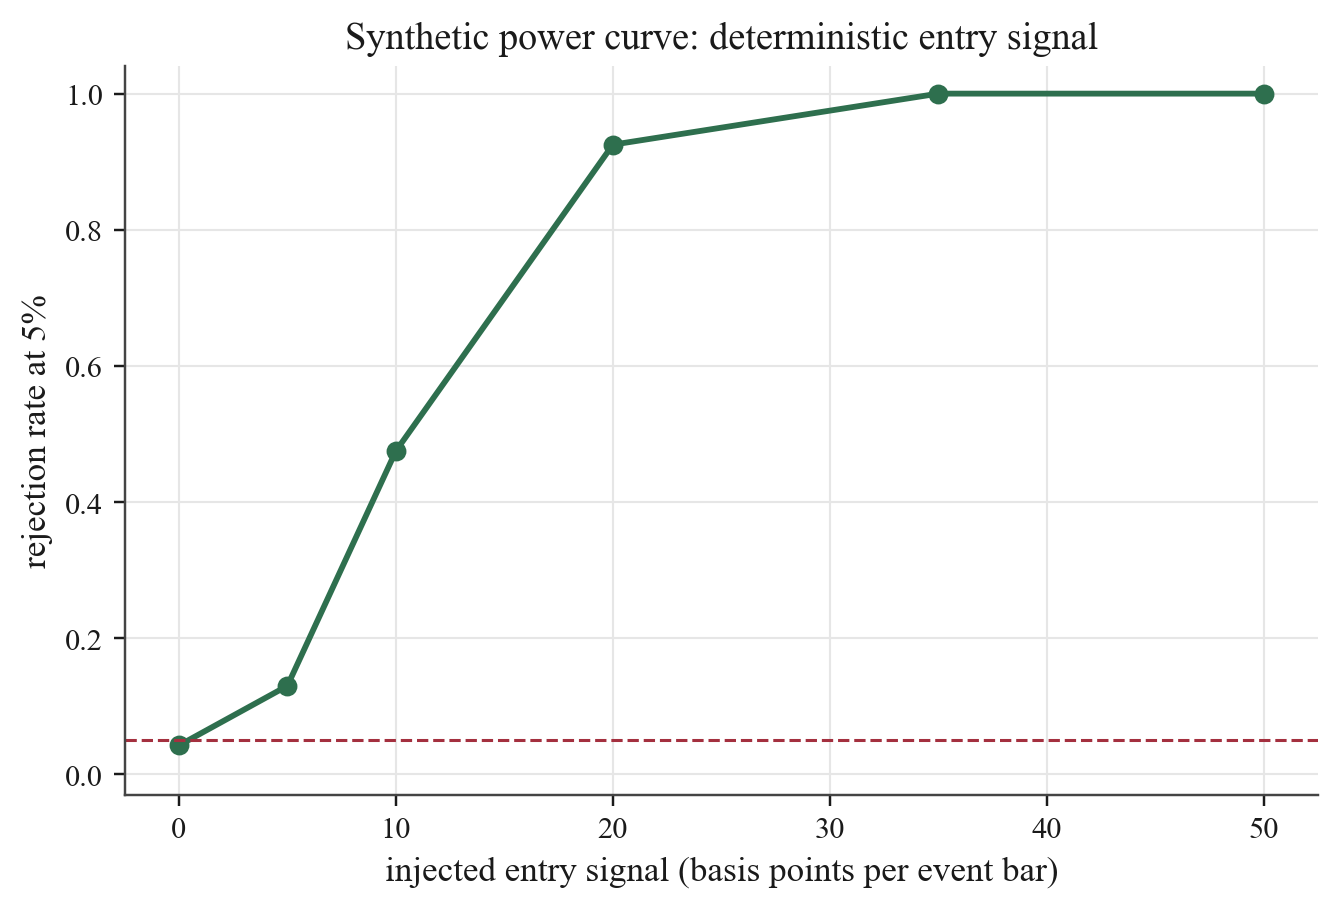
\includegraphics[width=0.78\textwidth]{synthetic_power_curve.png}
\caption{Synthetic power curve for deterministic entry signal. Signal strength is measured in basis points added to each event-window return bar.}
\label{fig:synthetic_power}
\end{figure}

\subsection{Positive control: detecting injected skill on the real price path}
\label{sec:positive-control}

The synthetic worlds above establish calibration and power in artificial data. A sharper question is whether the test can ever reject on the \emph{real} GC=F price path, or whether the null verdict merely reflects a procedure incapable of rejection. We answer this directly with a positive control. On the actual GC=F open-price series we construct a long-only strategy of $N=30$ trades, each held $d=10$ open-to-open bars at equal weight, and we control its timing quality with a skill parameter $\alpha\in[0,1]$. Here, a fraction $\alpha$ of entries are placed, using forward information, in the top quintile of the $d$-bar forward-return distribution available in their local feasible window (``good timing''), and the remaining $1-\alpha$ are placed by an unbiased random non-overlapping draw (``luck''). At $\alpha=0$ the strategy carries no timing skill; at $\alpha=1$ every entry is well timed. The oracle uses future information \emph{by construction}; we are careful to flag that it is an injected control, not a claim that any gold trader possesses such foresight. We then score each realized schedule against the paper's own structure-preserving null (Section~\ref{sec:spr}), which preserves the realized durations and gap multiset and randomizes only placement, because that is precisely what destroys the oracle alignment. We compute the realized statistic and the null with execution-cost simulation disabled, so the two differ only in placement; we run $100$ seeds per skill level at $M=5{,}000$ simulations.

\begin{table}[H]
\centering
\caption{Positive control on the real GC=F price path: detection of injected entry-placement skill. A fraction $\alpha$ of the $30$ long trades are placed with genuine foresight; the rest are random. Each row averages $100$ seeds at $M=5{,}000$ structure-preserving null simulations. ``Reject @ 5\%'' and ``Strong rate'' are the shares of seeds with $p\le0.05$ and with a Strong-skill classification respectively.}
\label{tab:positive_control}
{\small
\renewcommand{\arraystretch}{1.12}
\begin{adjustbox}{max width=\textwidth}
\begin{tabular}{@{}rrrrrrr@{}}
\toprule
Injected skill $\alpha$ & Mean $p$ & Median $p$ & Mean percentile & Mean $\mathrm{RCSI}_z$ & Reject @ 5\% & Strong rate \\
\midrule
0.00 & 0.495 & 0.530 & \phantom{0}50.5 & 0.03 & 0.03 & 0.03 \\
0.20 & 0.158 & 0.091 & \phantom{0}84.2 & 1.38 & 0.35 & 0.22 \\
0.40 & 0.021 & 0.002 & \phantom{0}98.0 & 2.91 & 0.88 & 0.81 \\
0.60 & 0.002 & $<0.001$ & \phantom{0}99.8 & 4.46 & 0.99 & 0.98 \\
0.80 & $<0.001$ & $<0.001$ & 100.0 & 5.84 & 1.00 & 1.00 \\
1.00 & $<0.001$ & $<0.001$ & 100.0 & 7.23 & 1.00 & 1.00 \\
\bottomrule
\end{tabular}
\end{adjustbox}
}
\par\vspace{0.5em}
\begin{minipage}{0.95\textwidth}
\centering
\footnotesize\emph{Notes.} $\alpha=0$ is a genuine no-skill control: it sits at the null median ($50$th percentile, $\mathrm{RCSI}_z\approx0$) and rejects within Monte Carlo error of the nominal $5\%$ rate. Median $p$ reaches the $1/(M+1)$ resolution floor at high $\alpha$.
\end{minipage}
\end{table}

The control behaves exactly as a sound test should (Table~\ref{tab:positive_control}, Figure~\ref{fig:pc_curve}). With no injected skill the test sits squarely at the null median ($50.5$th percentile, mean $\mathrm{RCSI}_z$ of $0.03$) and rejects within Monte Carlo error of the nominal $5\%$ rate. As genuine timing skill is added, power rises monotonically: by $\alpha=0.4$, $88\%$ of seeds reject and $81\%$ are classified Strong, and by $\alpha\ge0.8$ every seed is Strong, with mean $\mathrm{RCSI}_z$ climbing from $2.9$ at $\alpha=0.4$ to $7.2$ at $\alpha=1$. Figure~\ref{fig:pc_hist} shows a single well-timed run ($\alpha=1$): its realized cumulative return falls far in the upper tail of the structure-preserving null ($p\approx0.0002$, $\mathrm{RCSI}_z\approx8$), with no random placement of the same trades coming close. This shows that the null result reported for the real strategies is not an artifact of a powerless test on real prices; when entry-placement skill is genuinely present on the GC=F path, this procedure detects it. Repeating the control with stochastic execution costs enabled ($20$ seeds; \texttt{Data\_Clean/GC=F\_positive\_control\_power\_costson\_summary.csv}) leaves detection unchanged: the size is held at $\alpha=0$ (rejection within Monte Carlo error of $5\%$), every seed rejects by an injected-skill fraction of $0.4$, and mean $\mathrm{RCSI}_z$ rises to $7.2$ at full skill. Detection is therefore driven by the placement signal rather than by the cost treatment.

\begin{figure}[htbp]
\centering
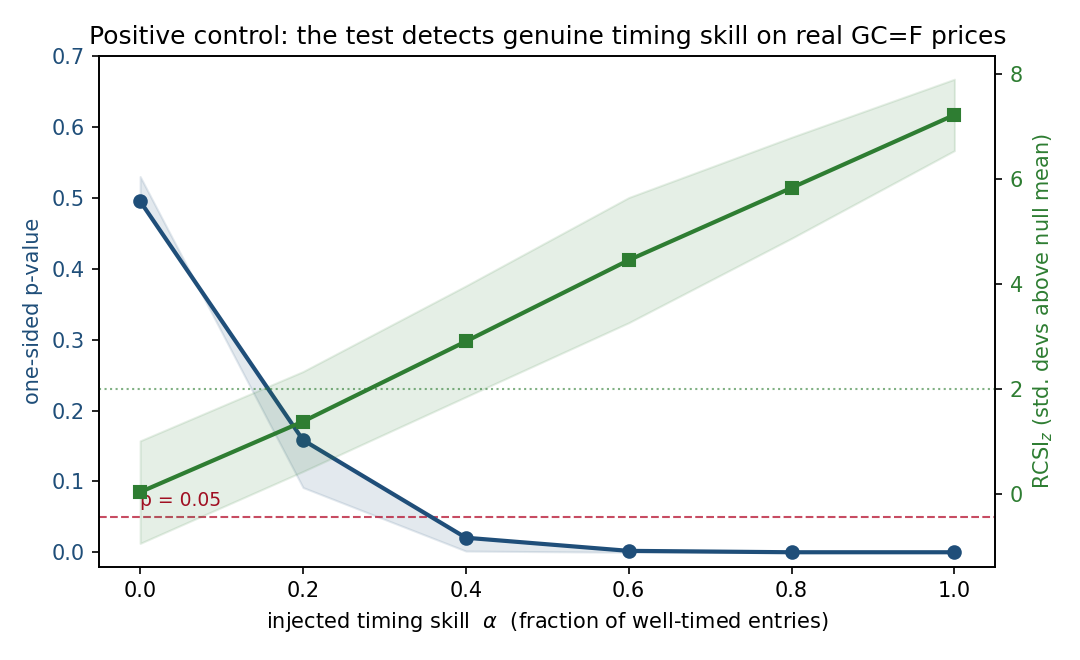
\includegraphics[width=0.82\textwidth]{positive_control_skill_curve.png}
\caption{Positive control on real GC=F prices. As injected timing skill $\alpha$ increases, the mean one-sided $p$-value (blue, left axis) collapses below $0.05$ and the mean $\mathrm{RCSI}_z$ (green, right axis) rises well past $2$. Bands show the seed dispersion. At $\alpha=0$ the test behaves like the null.}
\label{fig:pc_curve}
\end{figure}

\begin{figure}[htbp]
\centering
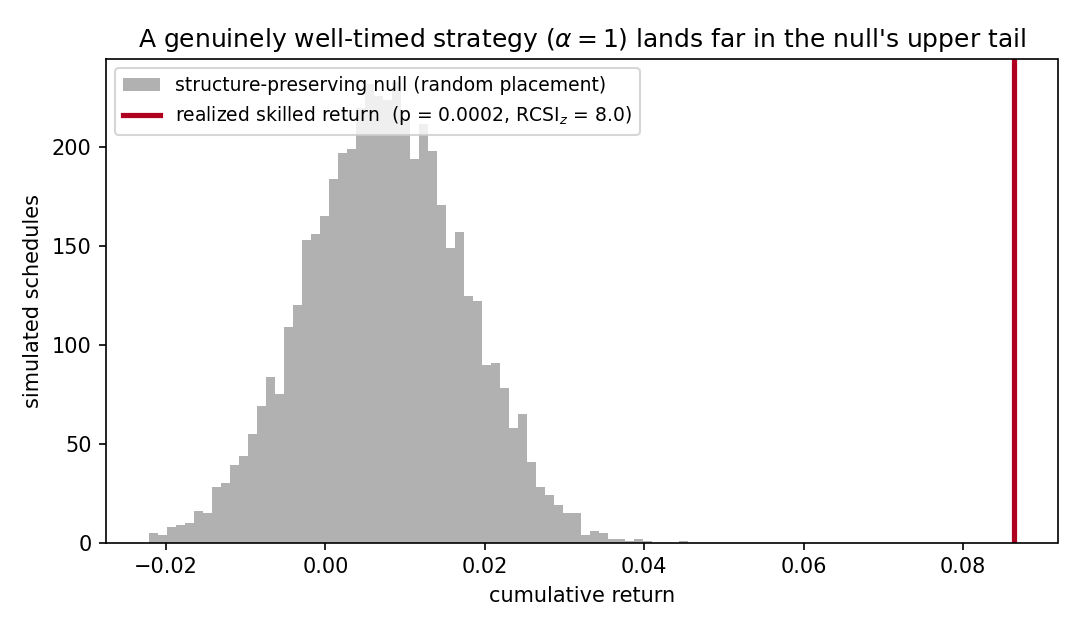
\includegraphics[width=0.82\textwidth]{positive_control_example_histogram.png}
\caption{A single genuinely well-timed strategy ($\alpha=1$) on the real GC=F path. The realized cumulative return (red) lies far beyond the entire structure-preserving null distribution of the same trades placed at random ($p\approx0.0002$, $\mathrm{RCSI}_z\approx8$).}
\label{fig:pc_hist}
\end{figure}

\subsection{Detecting realistic and imperfect signals}
\label{sec:realistic-signals}

The oracle of the previous subsection uses future information by construction, so it certifies only that the test \emph{can} reject; the relevant question is whether it detects the noisy, imperfect signals a real strategy would use. We answer this on the same GC=F path by driving entry placement with signals of controlled quality, summarized by $\rho$, the Pearson correlation between the entry signal and the $d$-bar forward return. A strategy enters at its top-$N$ signal bars (mutually non-overlapping), and we score the realized schedule against the same structure-preserving null. Here, the oracle is the limiting case $\rho\to1$ and $\rho=0$ is no skill.

Figure~\ref{fig:signal_curve} reports power as a function of realized signal quality, using a noisy signal $s=z(f)+\lambda\varepsilon$ whose correlation with the forward return $f$ we tune across a grid. The rejection rate rises smoothly from the nominal $5\%$ level at $\rho\approx0$ ($\rho=0.0001$: reject rate $0.00$, mean $p=0.52$) to certain detection by $\rho\approx0.20$ (reject rate $1.00$, mean $p=0.005$), passing through partial power at $\rho\approx0.10$ (reject rate $0.48$, mean $p=0.099$). The minimum detectable signal--return correlation for $80\%$ power is therefore roughly $\rho\approx0.15$ at the GC=F trade counts. This is a concrete, interpretable sensitivity that the bare oracle does not provide, and it matches the $\sqrt{N_s}$ scaling of Section~\ref{sec:theory}.

\begin{figure}[htbp]
\centering
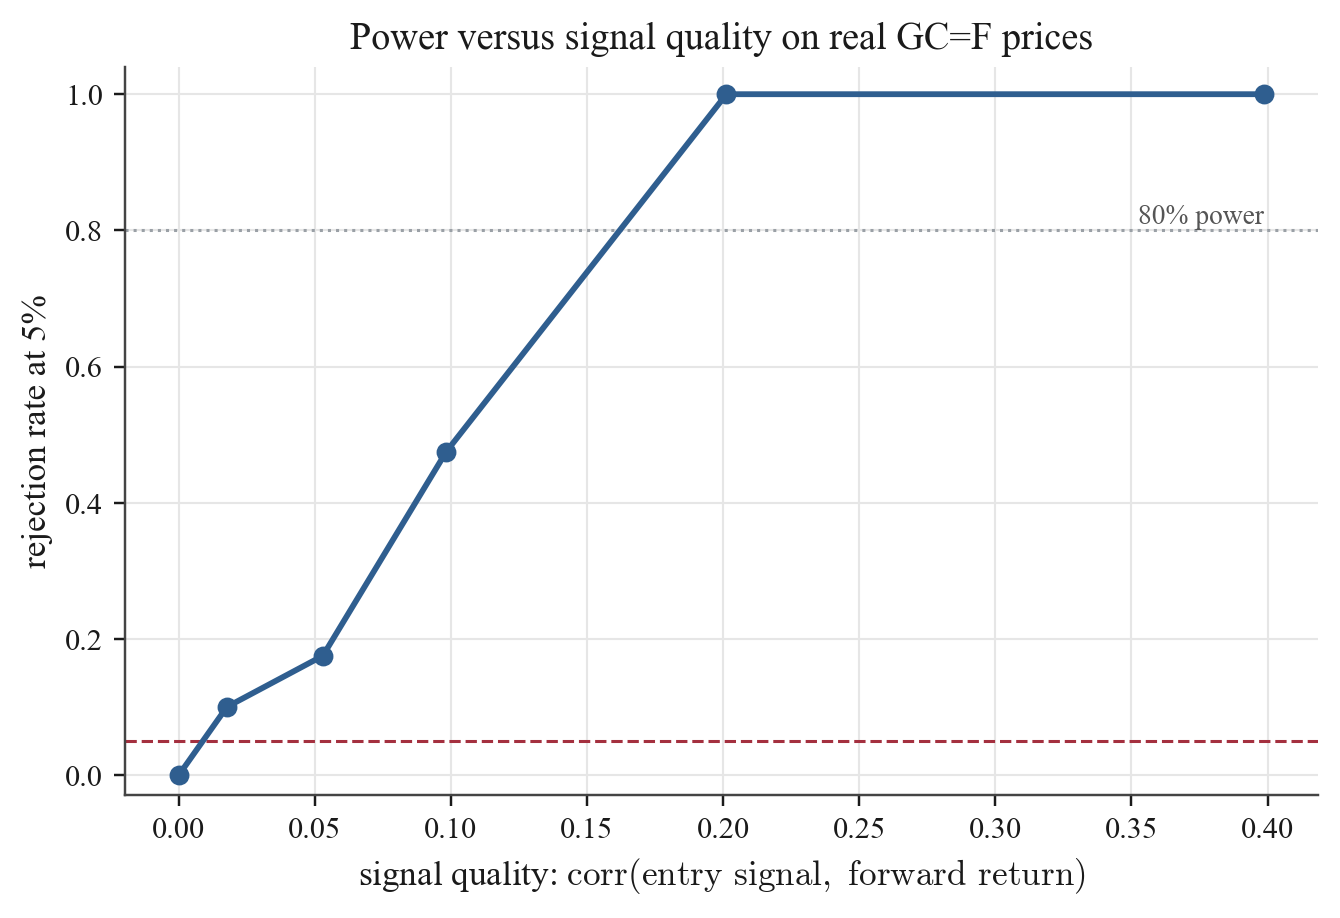
\includegraphics[width=0.74\textwidth]{positive_control_signal_curve.png}
\caption{Power versus signal quality on the real GC=F path. Each point averages $40$ seeds at $M=5{,}000$; the horizontal lines mark the nominal $5\%$ level and $80\%$ power. Rejection rises smoothly with the realized signal--forward-return correlation, giving a minimum detectable correlation of roughly $0.15$.}
\label{fig:signal_curve}
\end{figure}

Detection does not depend on foresight or on a particular signal-generating process. Table~\ref{tab:signal_mechanisms} applies the test to four mechanisms: a noisy oracle, an AR(1)-smoothed signal, a regime-conditional signal (skill only inside calm regimes), and a \emph{causal} momentum signal (trailing return, using no future information). The three signals with positive realized quality are detected in proportion to their correlation: regime-conditional ($\rho=0.27$) most strongly, then AR(1) ($\rho=0.16$) and the noisy oracle ($\rho=0.10$). The momentum signal is the most instructive. On gold at this horizon, trailing momentum is \emph{anti}-correlated with the forward return ($\rho=-0.07$, a mean-reverting tendency), so it times entries poorly, and the test correctly assigns it no skill; indeed it sits well below the null median. The procedure therefore responds to the realized informativeness of a signal, not to the analyst's intent or to whether the signal is causal.

\begin{table}[H]
\centering
\caption{Detection across signal-generating processes on the real GC=F path (target correlation $0.10$ for the calibrated signals; $40$ seeds at $M=5{,}000$). $\bar\rho$ is the mean realized signal--forward-return correlation.}
\label{tab:signal_mechanisms}
{\small
\renewcommand{\arraystretch}{1.12}
\begin{adjustbox}{max width=\textwidth}
\begin{tabular}{@{}lrrrr@{}}
\toprule
Signal-generating process & $\bar\rho$ & Mean $p$ & Reject @ 5\% & Mean $\mathrm{RCSI}_z$ \\
\midrule
Regime-conditional (calm-only skill) & \phantom{-}0.27 & 0.054 & 0.85 & \phantom{-}2.42 \\
AR(1)-smoothed signal & \phantom{-}0.16 & 0.051 & 0.63 & \phantom{-}2.15 \\
Noisy oracle & \phantom{-}0.10 & 0.107 & 0.40 & \phantom{-}1.49 \\
Momentum, causal (trailing return) & $-0.07$ & 1.000 & 0.00 & $-4.82$ \\
\bottomrule
\end{tabular}
\end{adjustbox}
}
\par\vspace{0.5em}
\begin{minipage}{0.95\textwidth}
\centering
\footnotesize\emph{Notes.} Calibrated signals (noisy oracle, AR(1)) target a modest correlation of $0.10$; the regime-conditional and causal-momentum signals realize whatever correlation the data produce. A causal momentum rule is anti-predictive for entry timing on gold at the $10$-bar horizon, and is correctly classified below the null median rather than as skill.
\end{minipage}
\end{table}


\section{Additional empirical analyses}
\label{supp:additional}

\subsection{Cross-asset breadth under multiplicity control}
\label{sec:supp-cross-asset}

The walk-forward panel above tests temporal stability within a curated set of instruments. A complementary question is what happens when every completed full-sample test is pooled and judged jointly, with explicit correction for the fact that many tests are being run at once. We aggregate the structure-preserving Monte Carlo result for every strategy on every asset for which a completed run exists on disk: $322$ strategy-by-asset tests across $47$ instruments spanning equities, ETFs, futures, commodities, FX, and crypto. This is a search for skill at breadth: if entry-placement edge existed broadly in this universe a naive scan would tend to find it, and we make that scan honest by imposing multiplicity control.

\begin{table}[H]
\centering
\caption{Cross-asset panel under multiplicity control. Every completed structure-preserving test on disk is pooled and corrected jointly. ``Nominal'' counts raw $p\le0.05$; BH and Bonferroni control the false discovery rate and family-wise error rate at $0.05$ across all $322$ tests.}
\label{tab:cross_asset_multiplicity}
{\small
\renewcommand{\arraystretch}{1.12}
\begin{adjustbox}{max width=\textwidth}
\begin{tabular}{@{}lr@{}}
\toprule
Quantity & Value \\
\midrule
Assets / strategy-by-asset tests & $47$ / $322$ \\
Nominal rejections at $p\le0.05$ & $13$ (vs.\ $16.1$ expected by chance) \\
Benjamini--Hochberg discoveries (FDR $0.05$) & $0$ \\
Bonferroni discoveries (FWER $0.05$, threshold $1.55\times10^{-4}$) & $0$ \\
Mean / median panel $p$-value & $0.567$ / $0.580$ \\
KS statistic vs.\ Uniform$(0,1)$ (departure direction) & $0.114$ (conservative) \\
Smallest $p$-value in the panel & $0.0014$ (a \emph{random}-entry baseline) \\
\bottomrule
\end{tabular}
\end{adjustbox}
}
\par\vspace{0.5em}
\begin{minipage}{0.95\textwidth}
\centering
\footnotesize\emph{Notes.} The panel $p$-values skew conservative (mean $0.567>0.5$): there are \emph{fewer} small $p$-values than chance ($13$ vs.\ $16.1$ at the $5\%$ level; $4.0\%$ vs.\ $5\%$) and an excess of large ones, so the KS departure from uniformity is in the conservative direction, not toward hidden signal. The random-entry baseline is included as one strategy per asset.
\end{minipage}
\end{table}

At breadth, nothing survives multiplicity control. After Benjamini--Hochberg or Bonferroni correction there are zero discoveries across all $322$ tests, and the raw count of nominal rejections ($13$) is below the $16.1$ expected under a global no-skill null. The panel $p$-values are not merely consistent with that null but skew conservative; their mass concentrates at high values (mean $0.567$), which is what a deficit of genuine timing skill, net of transaction costs, produces. The most direct evidence that the nominal hits are luck rather than skill is the identity of the strategies producing them: the single smallest $p$-value in the entire panel ($0.0014$) belongs to a \emph{random}-entry baseline on DIA, a random baseline holds the second-largest $\mathrm{RCSI}_z$ of all $322$ tests, and random baselines occupy three of the thirteen nominal rejections. A diagnostic whose top-ranked strategies are random baselines is recovering chance rather than edge. Figure~\ref{fig:cross_asset} shows both facts at once: the $p$-value histogram tilts conservative, and on the Benjamini--Hochberg plot every ordered $p$-value, random baselines included, sits well above the rejection line.

\begin{figure}[htbp]
\centering
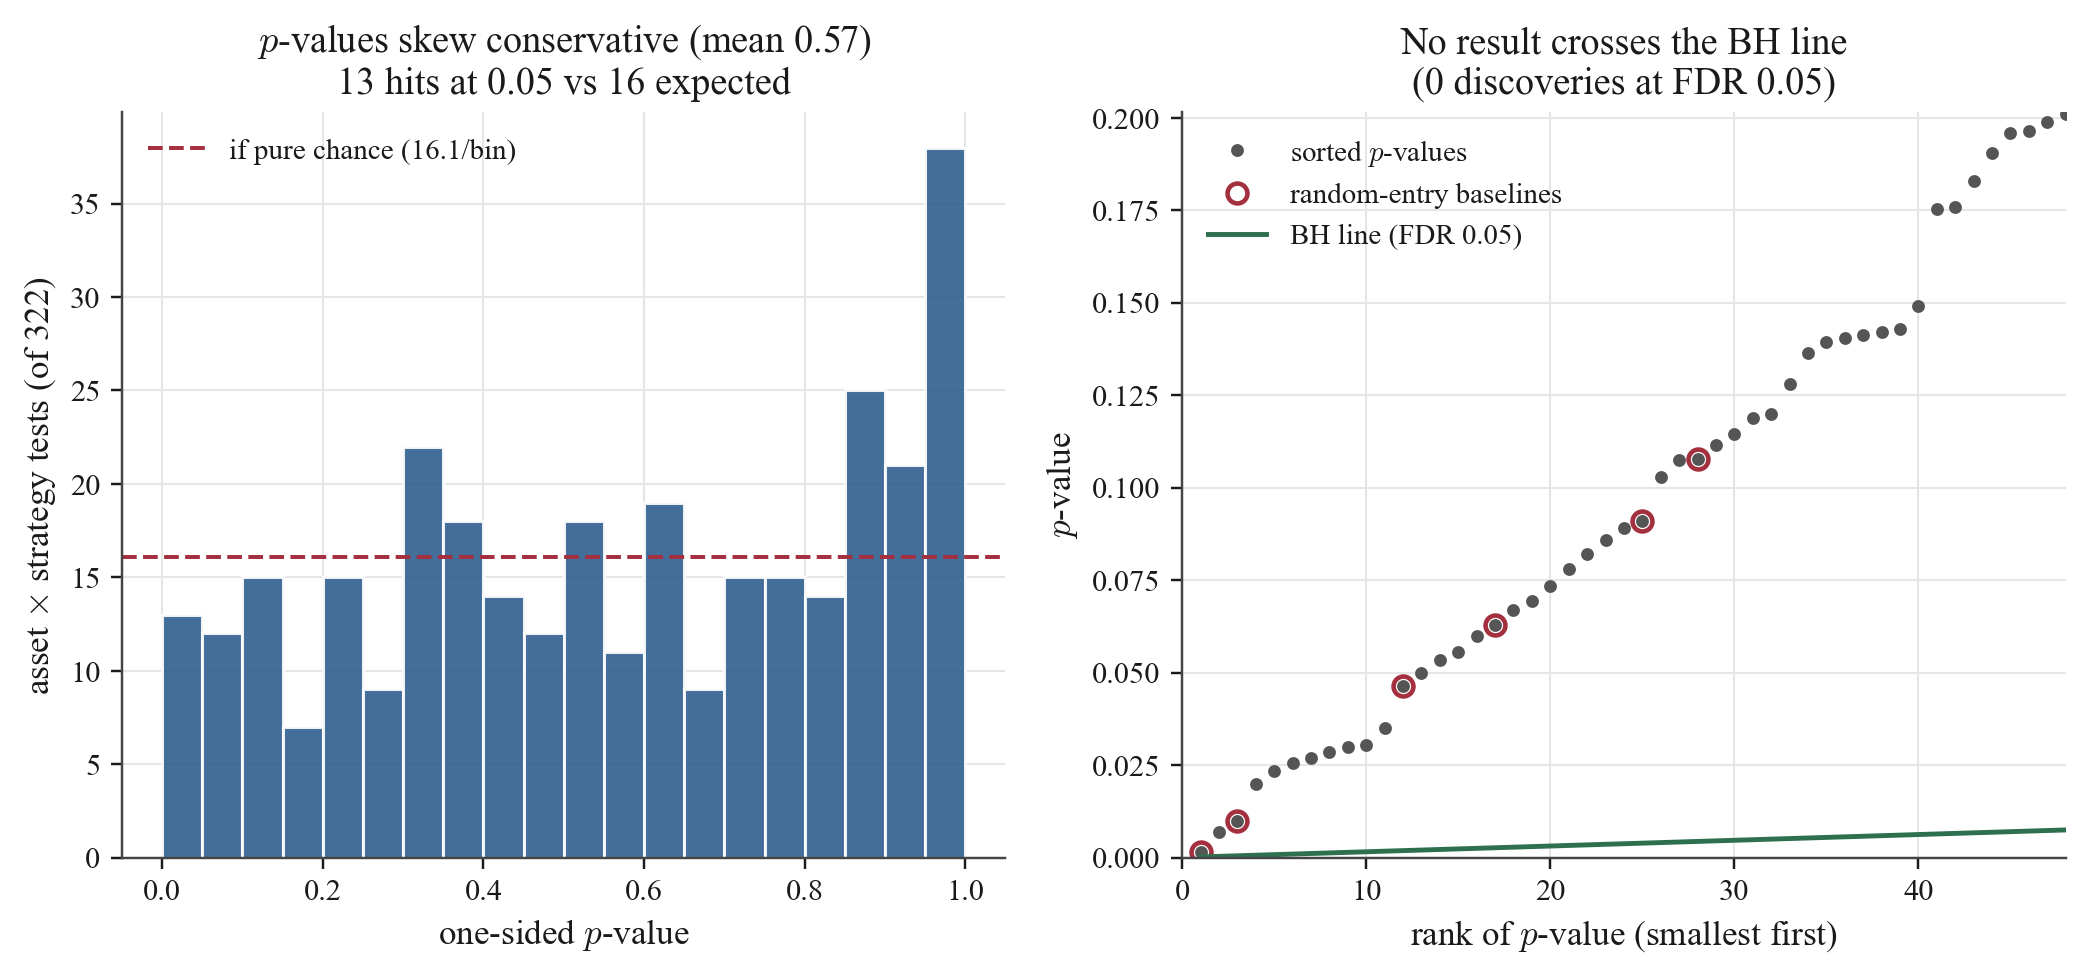
\includegraphics[width=0.95\textwidth]{cross_asset_multiplicity.png}
\caption{Cross-asset panel of $322$ structure-preserving tests across $47$ instruments. Left: the $p$-value histogram skews conservative, with $13$ nominal rejections versus $16.1$ expected by chance. Right: the Benjamini--Hochberg plot. No ordered $p$-value crosses the FDR line, so there are zero discoveries; circled points are random-entry baselines, which sit among the smallest $p$-values.}
\label{fig:cross_asset}
\end{figure}

\paragraph{What the panel is, and is not.} Three selection questions deserve direct answers. First, on \emph{strategy choice}: the eleven-rule panel is fixed, with thresholds set ex ante (\ref{app:strategy_rules}) and applied identically to every asset; there is no per-asset re-optimization, so the within-scan researcher degrees of freedom are confined to the asset universe rather than the rules. Second, on \emph{asset choice}: the $47$ instruments are those for which a completed structure-preserving run existed, an availability sample spanning equity ETFs, single names, futures, commodities, FX, and crypto, not a set curated on outcomes. We report every test that exists rather than a selected subset, and the embedded random-entry baselines act as a built-in negative control, because any selection or specification artifact that inflated significance would inflate the baselines too, and it does not. Third, on \emph{survivorship}: the universe contains currently traded instruments, so delisted names are absent. This cannot manufacture the finding, for two reasons. First, the result is a \emph{null}, and survivorship would if anything bias toward detecting skill (survivors trend upward). Second, the structure-preserving null absorbs that drift by construction, because it reprices the same trades on the same surviving path. We are careful not to overstate the design: the honest characterization is a pooled, dependence-laden convenience sample (correlated assets and shared strategy logic) analyzed with dependence-aware multiplicity control \cite{benjaminihochberg1995,BenjaminiYekutieli2001}, not a designed-universe study. We present it as breadth evidence against the existence of broad, easily found timing skill, not as a representative census.

\subsection{Comparison to alternative nulls}

To show what the structure-preserving null adds, we re-evaluate the empirical panel against two return-based baselines. The shuffled-return null replays each realized trade schedule on IID permutations of the observed open-to-open returns. The stationary-bootstrap null replays the same schedules on stationary-bootstrap return paths with mean block length 20 bars. Both preserve the realized trade geometry but replace the realized price path; this means they isolate the price path as the only thing that changes. We run the comparison with fixed transaction cost $c=0.000470$, $M=5{,}000$ simulations per strategy and method (Table~\ref{tab:null_benchmark}).

\begin{table}[H]
\centering
\caption{Comparison of null methods on the GC=F strategy panel.}
\label{tab:null_benchmark}
{\small
\renewcommand{\arraystretch}{1.12}
\begin{adjustbox}{max width=\textwidth}
\begin{tabular}{@{}lccccrrl@{}}
\toprule
Null method & Path & Geometry & Snooping & Entry test & Median $p$ & Reject @ 5\% & Closest strategy \\
\midrule
Structure-preserving schedule & Yes & Yes & No & Yes & 0.348 & 0 & Squeeze Breakout ($p=0.058$) \\
Shuffled returns & No & Yes & No & No & 0.293 & 1 & Squeeze Breakout ($p=0.030$) \\
Stationary bootstrap returns & No & Yes & No & No & 0.309 & 1 & Squeeze Breakout ($p=0.025$) \\
\bottomrule
\end{tabular}
\end{adjustbox}
}
\par\vspace{0.5em}
\begin{minipage}{0.95\textwidth}
\centering
\footnotesize\emph{Notes.} ``Path'' indicates whether the realized price path is preserved. ``Geometry'' indicates whether realized entries, exits, holding periods, weights, and directions are retained or structurally matched. ``Snooping'' indicates whether the method controls strategy-selection search across the panel; none of these within-strategy diagnostics does so. Method-specific Benjamini--Hochberg adjustment leaves no strategy significant at 5\% under any method. The structure-preserving-schedule row is computed by the independent benchmark-comparison harness ($M=5{,}000$, separate seed); its Squeeze Breakout $p=0.058$ and median $p=0.348$ differ from the $0.053$ and $0.341$ of Table~\ref{tab:main} only by Monte Carlo seed variation.
\end{minipage}
\end{table}

\begin{figure}[htbp]
\centering
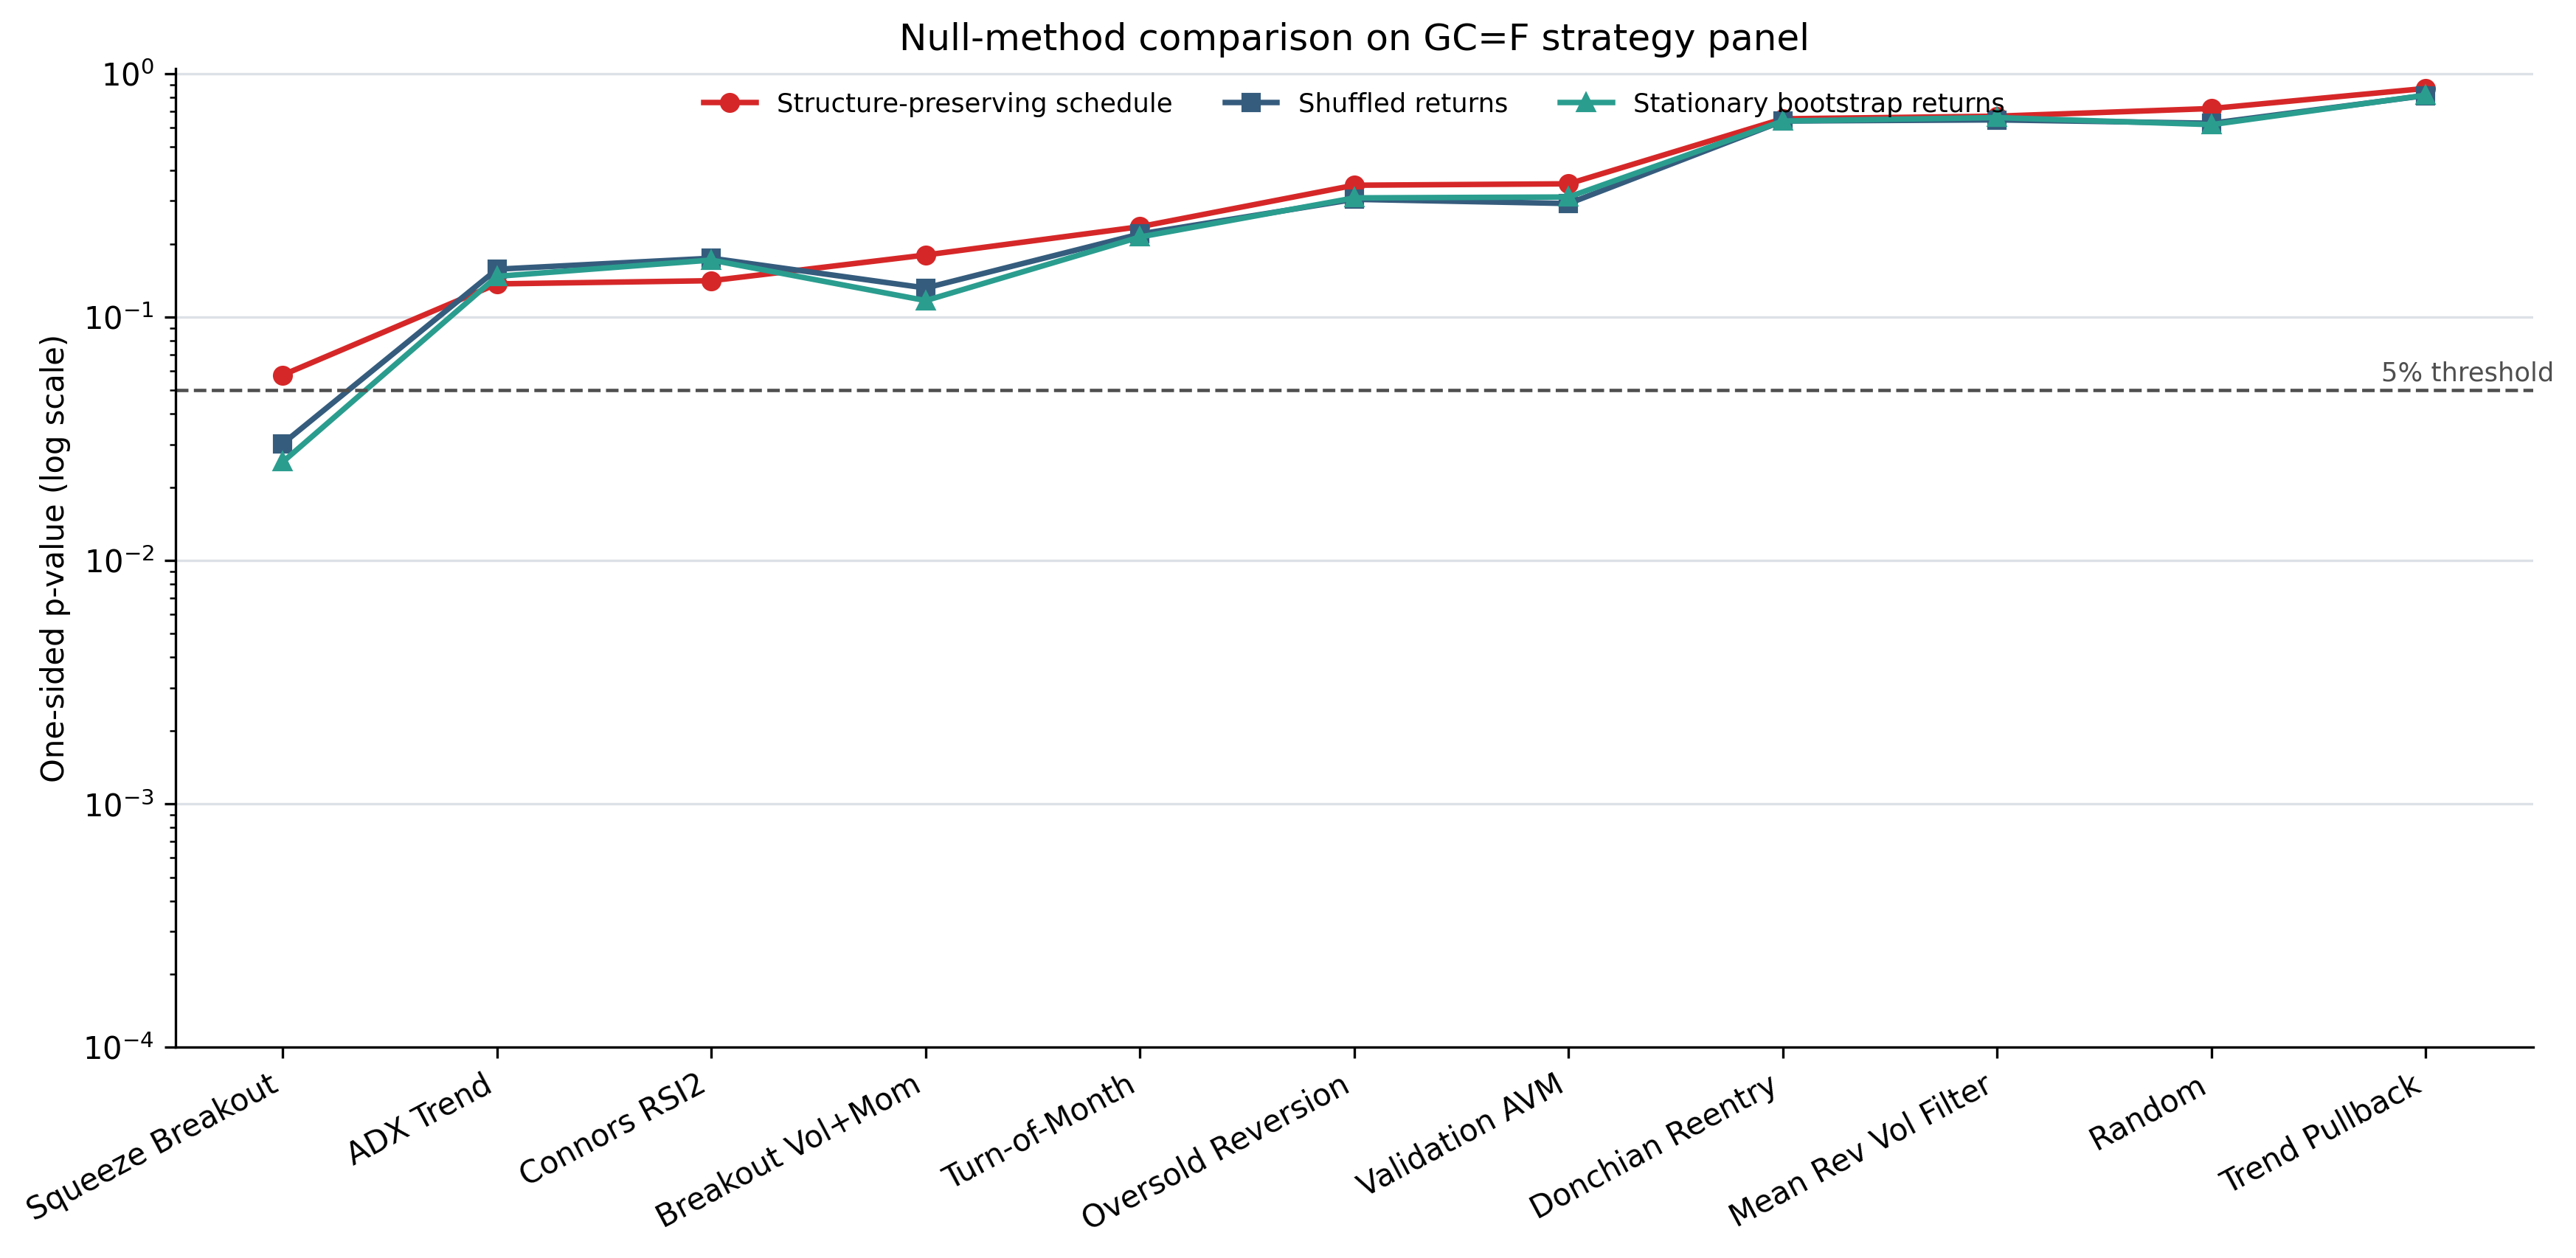
\includegraphics[width=0.95\textwidth]{null_method_comparison.png}
\caption{One-sided p-values under structure-preserving schedule randomization, shuffled returns, and stationary-bootstrap returns.}
\label{fig:null_method_comparison}
\end{figure}

The comparison clarifies the estimand (Figure~\ref{fig:null_method_comparison}). The return-based nulls make Squeeze Breakout significant at the raw 5\% level, while the structure-preserving schedule null leaves it just above threshold. This is not a contradiction, because the two nulls ask different questions. The return nulls ask whether the realized trade schedule performs unusually well relative to synthetic return histories. The structure-preserving schedule null asks whether the realized entry placement is unusually good on the actual price path, conditional on the same exposure geometry. This means a strategy can look exceptional against resampled returns yet remain only marginal against randomized placement on the realized path. For this paper's question, the latter comparison is the one that targets placement on the realized path.

The benchmark also states plainly what remains unsolved. None of the three methods controls for the fact that the strategy panel itself was selected by the researcher. We do not claim to replace White's Reality Check or Hansen's SPA test; they answer the complementary between-strategy data-snooping question, which is a different problem from the one this diagnostic targets.

\subsection{Multi-asset walk-forward evidence}

We supplement the single-asset GC=F analysis with a daily multi-asset walk-forward panel. The universe contains equity ETFs (SPY, QQQ, VOO), single-name equities (AAPL, NVDA, TSM), futures and commodities (GC=F, CL=F, ES=F, NQ=F), foreign exchange (EURUSD=X, GBPUSD=X, AUDUSD=X), and crypto (BTC-USD). Each ticker is split into non-overlapping four-year test windows using 1{,}008-bar folds. We retain a strategy-fold panel only when it produces at least five trades, because a handful of trades cannot support a stable null. Each retained panel is evaluated with $M=1{,}000$ structure-preserving null simulations. This extension produces 712 strategy-fold panels (Table~\ref{tab:multi_asset_walk_forward}).

This section is exploratory. Unlike the GC=F robustness analysis, it uses one outer run per panel rather than repeated seed-level robustness, because the aim here is breadth rather than seed-robust precision. Its purpose is external-validity pressure: we are checking whether the main conclusion vanishes once the method leaves gold futures.

\begin{table}[H]
\centering
\caption{Daily multi-asset walk-forward panel summary.}
\label{tab:multi_asset_walk_forward}
{\small
\renewcommand{\arraystretch}{1.12}
\begin{adjustbox}{max width=\textwidth}
\begin{tabular}{@{}lrrrrrrl@{}}
\toprule
Strategy & Panels & Mean $p$ & Mean percentile & Mean $\mathrm{RCSI}_z$ & Sig.\ runs & Outperform null & Classification \\
\midrule
Trend Pullback      & 79 & 0.581 & 42.0 & -0.28 & 1.3\% & 40.5\% & Inconclusive \\
Breakout Vol+Mom    & 76 & 0.595 & 40.6 & -0.31 & 1.3\% & 36.8\% & Inconclusive \\
Mean Rev Vol Filter & 13 & 0.505 & 49.6 & \phantom{-}0.01 & 0.0\% & 38.5\% & Inconclusive \\
Validation AVM      & 73 & 0.599 & 40.2 & -0.33 & 2.7\% & 39.7\% & Inconclusive \\
ADX Trend           & 78 & 0.638 & 36.3 & -0.41 & 2.6\% & 29.5\% & Likely random \\
Oversold Reversion  & 69 & 0.515 & 48.6 & -0.11 & 1.4\% & 52.2\% & Inconclusive \\
Squeeze Breakout    & 24 & 0.691 & 31.0 & -0.59 & 0.0\% & 20.8\% & Likely random \\
Connors RSI2        & 76 & 0.493 & 50.8 & -0.06 & 5.3\% & 52.6\% & Inconclusive \\
Donchian Reentry    & 64 & 0.655 & 34.6 & -0.48 & 3.1\% & 25.0\% & Likely random \\
Turn-of-Month       & 80 & 0.567 & 43.4 & -0.26 & 3.8\% & 38.8\% & Inconclusive \\
Random              & 80 & 0.607 & 39.4 & -0.39 & 2.5\% & 36.3\% & Likely random \\
\bottomrule
\end{tabular}
\end{adjustbox}
}
\par\vspace{0.5em}
\begin{minipage}{0.95\textwidth}
\centering
\footnotesize\emph{Notes.} ``Sig.\ runs'' is the share of retained strategy-fold panels with $p\le0.05$ in the single outer run. ``Outperform null'' is the share whose realized cumulative return exceeds the null median. The run uses cached daily data, $M=1{,}000$ null simulations per panel, one outer run, and minimum five trades per retained panel.
\end{minipage}
\end{table}

\begin{figure}[htbp]
\centering
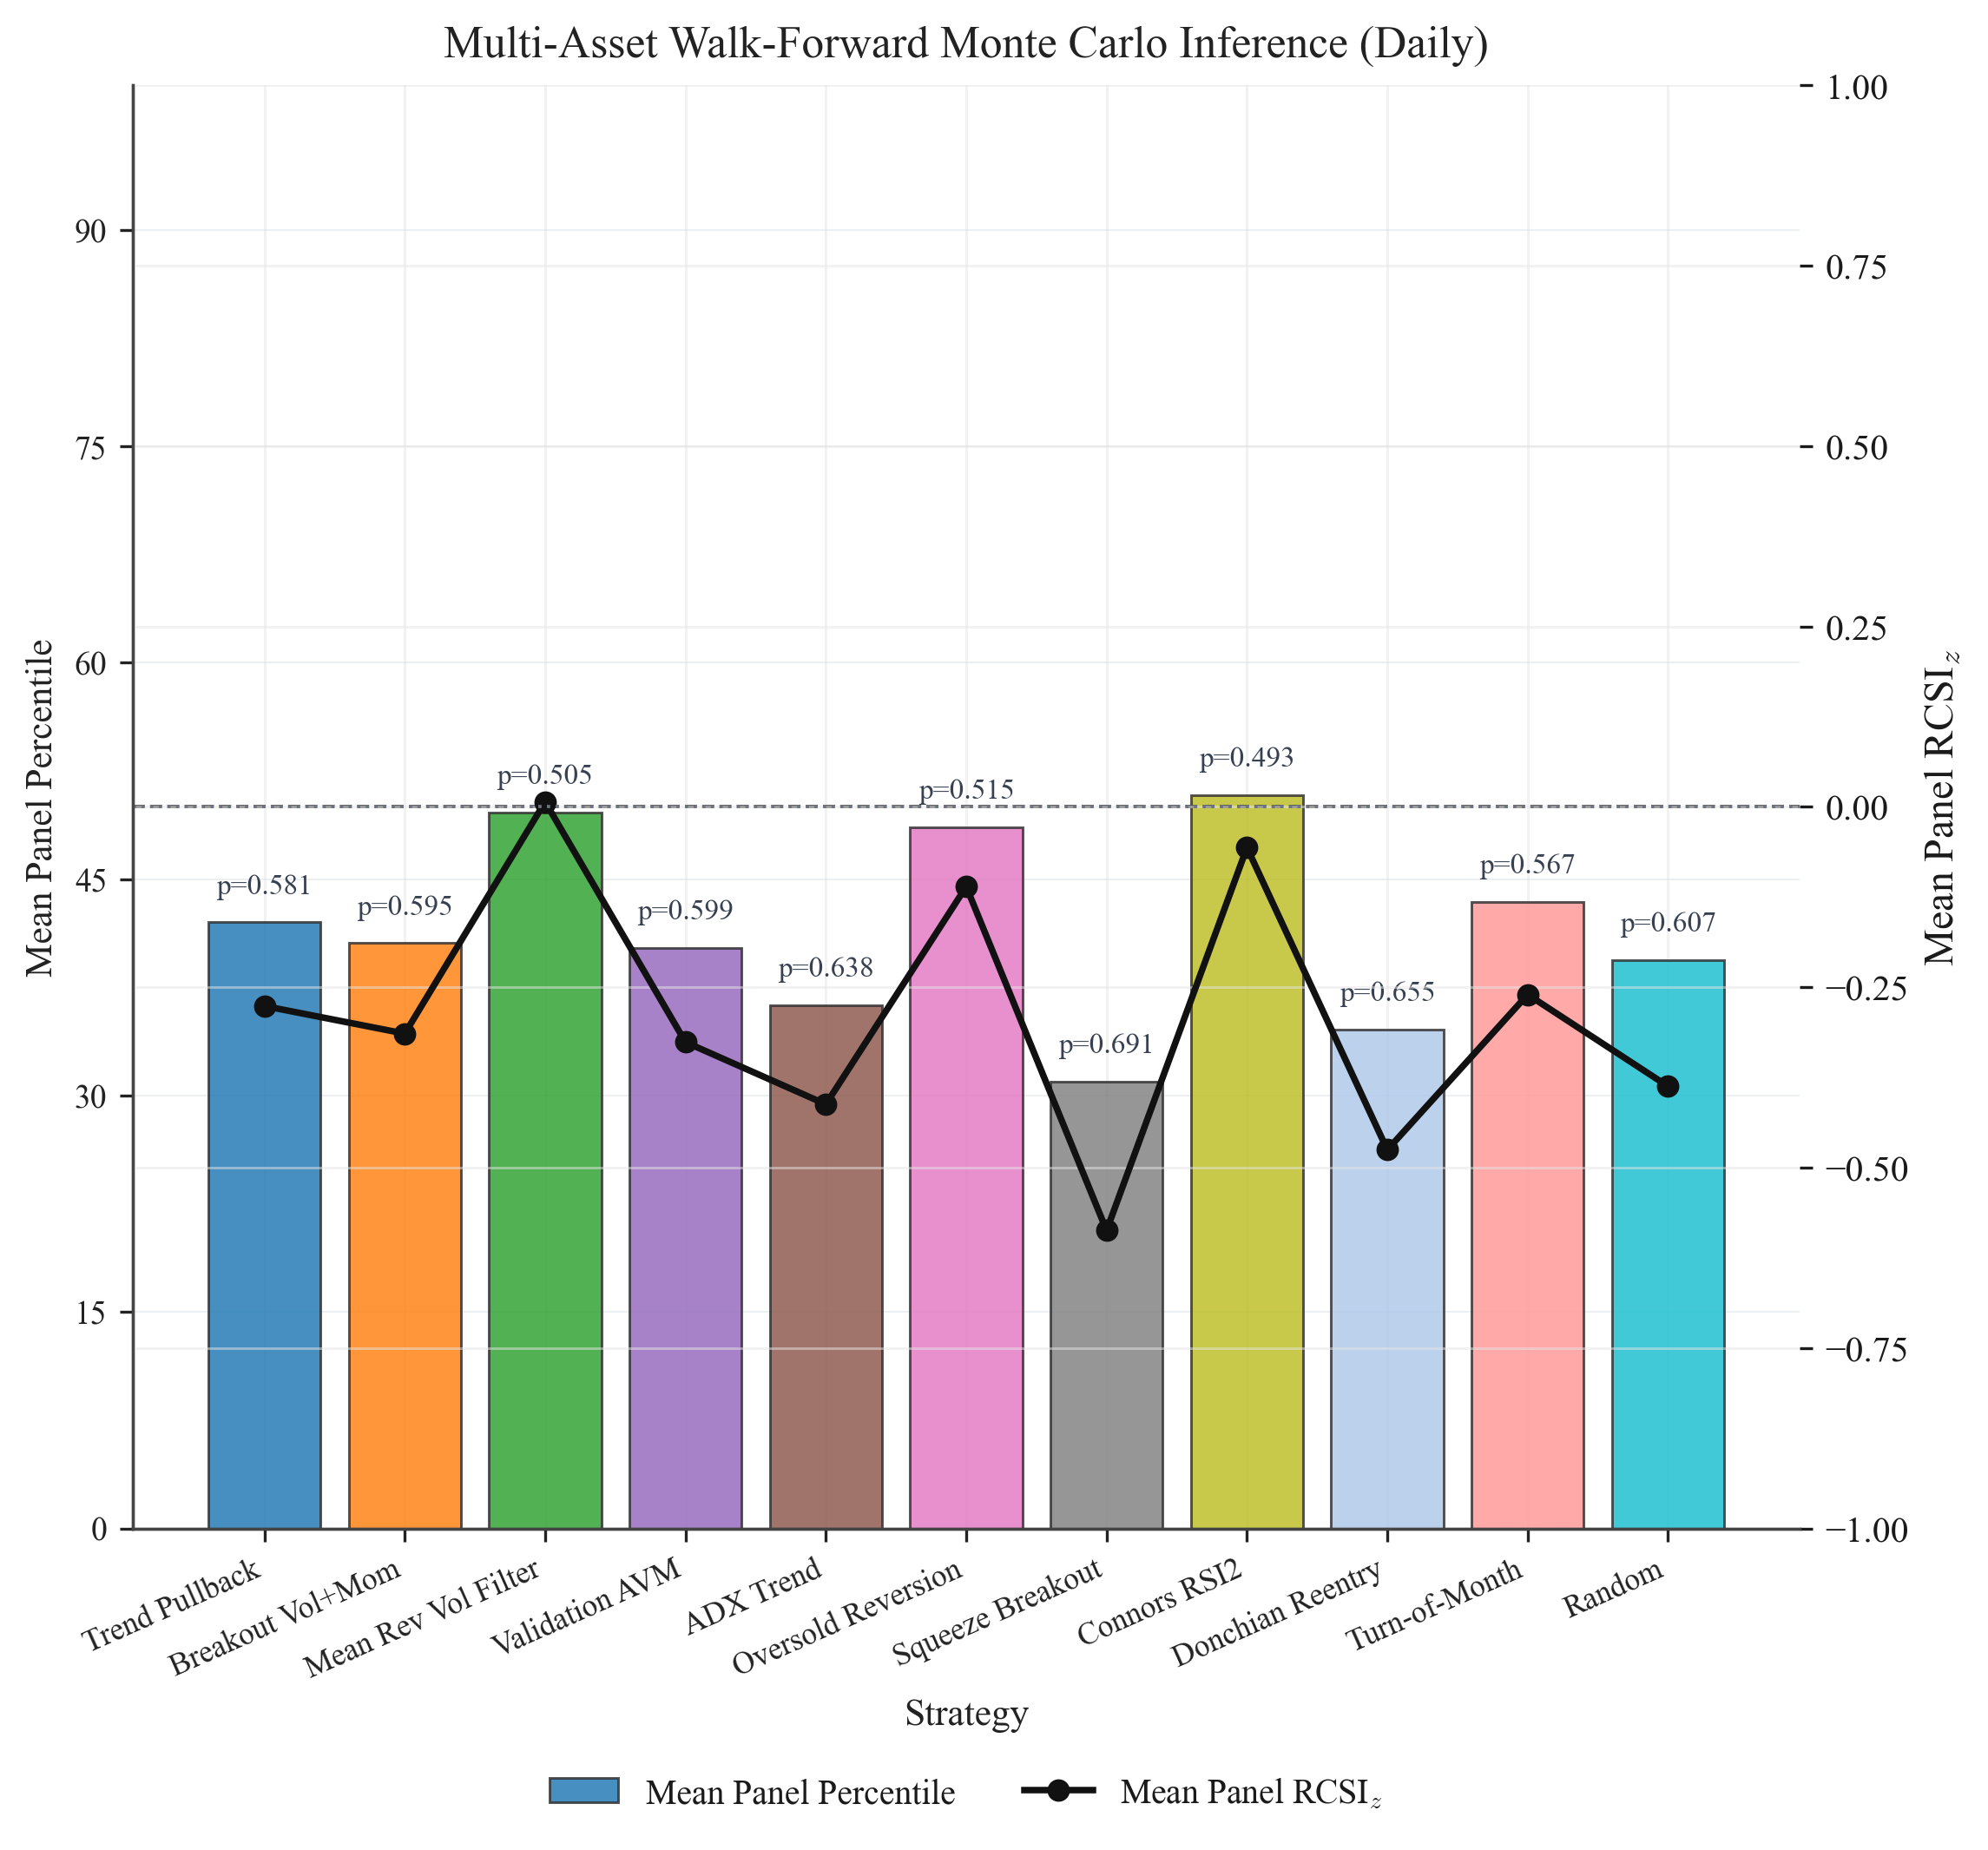
\includegraphics[width=0.95\textwidth]{multi_asset_walk_forward_inference.png}
\caption{Daily multi-asset walk-forward inference summary. Bars report mean panel percentile; the line reports mean panel $\mathrm{RCSI}_z$.}
\label{fig:multi_asset_inference}
\end{figure}

The multi-asset extension does not contradict the GC=F conclusion; still, as a single-outer-run panel it is exploratory and cannot independently confirm it, and seed-robust inference is established only for GC=F. No strategy has a mean panel $p$-value below 0.49. The strongest cross-panel percentile belongs to Connors RSI2 at 50.8, essentially the null median. Only Connors RSI2 exceeds the null median in more than half of retained panels, and only barely (52.6\%). Strategies that appeared weakly favorable in the single-asset analysis do not become broadly significant once evaluated across asset classes and non-overlapping walk-forward windows (Figure~\ref{fig:multi_asset_inference}).

We are careful not to overstate the result. Because the walk-forward extension uses one outer run per panel, it is not a replacement for the seed-robust GC=F Monte Carlo analysis. Still, it is useful evidence against the most serious external-validity objection: the paper is no longer only a gold-futures case study. The broader panel is consistent with the profit--skill divergence extending beyond GC=F.

\subsection{Frequency robustness check}
\label{sec:frequency-robustness}

We address the daily-only criticism with a bounded frequency-robustness check. We run the same walk-forward engine on SPY, QQQ, and BTC-USD at three bar intervals: daily, 4-hour, and hourly. To keep the comparison aligned with the shorter Yahoo Finance intraday history window, each interval uses at most the four most recent non-overlapping test folds per ticker. We scale the test windows to roughly the same calendar length, because otherwise the intervals would not be comparable: 126 daily bars, 252 four-hour bars, and 882 hourly bars. Each retained strategy-fold panel must contain at least five trades and is evaluated with $M=1{,}000$ structure-preserving null simulations and one outer run (Table~\ref{tab:frequency_robustness}).

\begin{table}[H]
\centering
\caption{Bounded frequency-robustness summary across SPY, QQQ, and BTC-USD.}
\label{tab:frequency_robustness}
{\small
\renewcommand{\arraystretch}{1.12}
\begin{adjustbox}{max width=\textwidth}
\begin{tabular}{@{}lrrrrrrl@{}}
\toprule
Interval & Strategies & Panels & Bars/fold & Min mean $p$ & Best percentile & Mean sig.\ panels & Best-percentile strategy \\
\midrule
Daily   & 6 & 18 & 126 & 0.244 & 75.7 & 0.0\% & Turn-of-Month \\
4-hour  & 5 & 10 & 252 & 0.593 & 40.8 & 0.0\% & Oversold Reversion \\
Hourly  & 5 & 15 & 882 & 0.236 & 76.5 & 4.0\% & Oversold Reversion \\
\bottomrule
\end{tabular}
\end{adjustbox}
}
\par\vspace{0.5em}
\begin{minipage}{0.95\textwidth}
\centering
\footnotesize\emph{Notes.} The panel uses the three tickers common to the daily, 4-hour, and hourly runs. ``Strategies'' counts strategies with at least one retained panel at that interval. ``Mean sig.\ panels'' averages the per-strategy share of retained panels with $p\le0.05$. The run is exploratory: one outer run, recent folds only, and sparse retained panels at higher frequencies.
\end{minipage}
\end{table}

\begin{figure}[htbp]
\centering
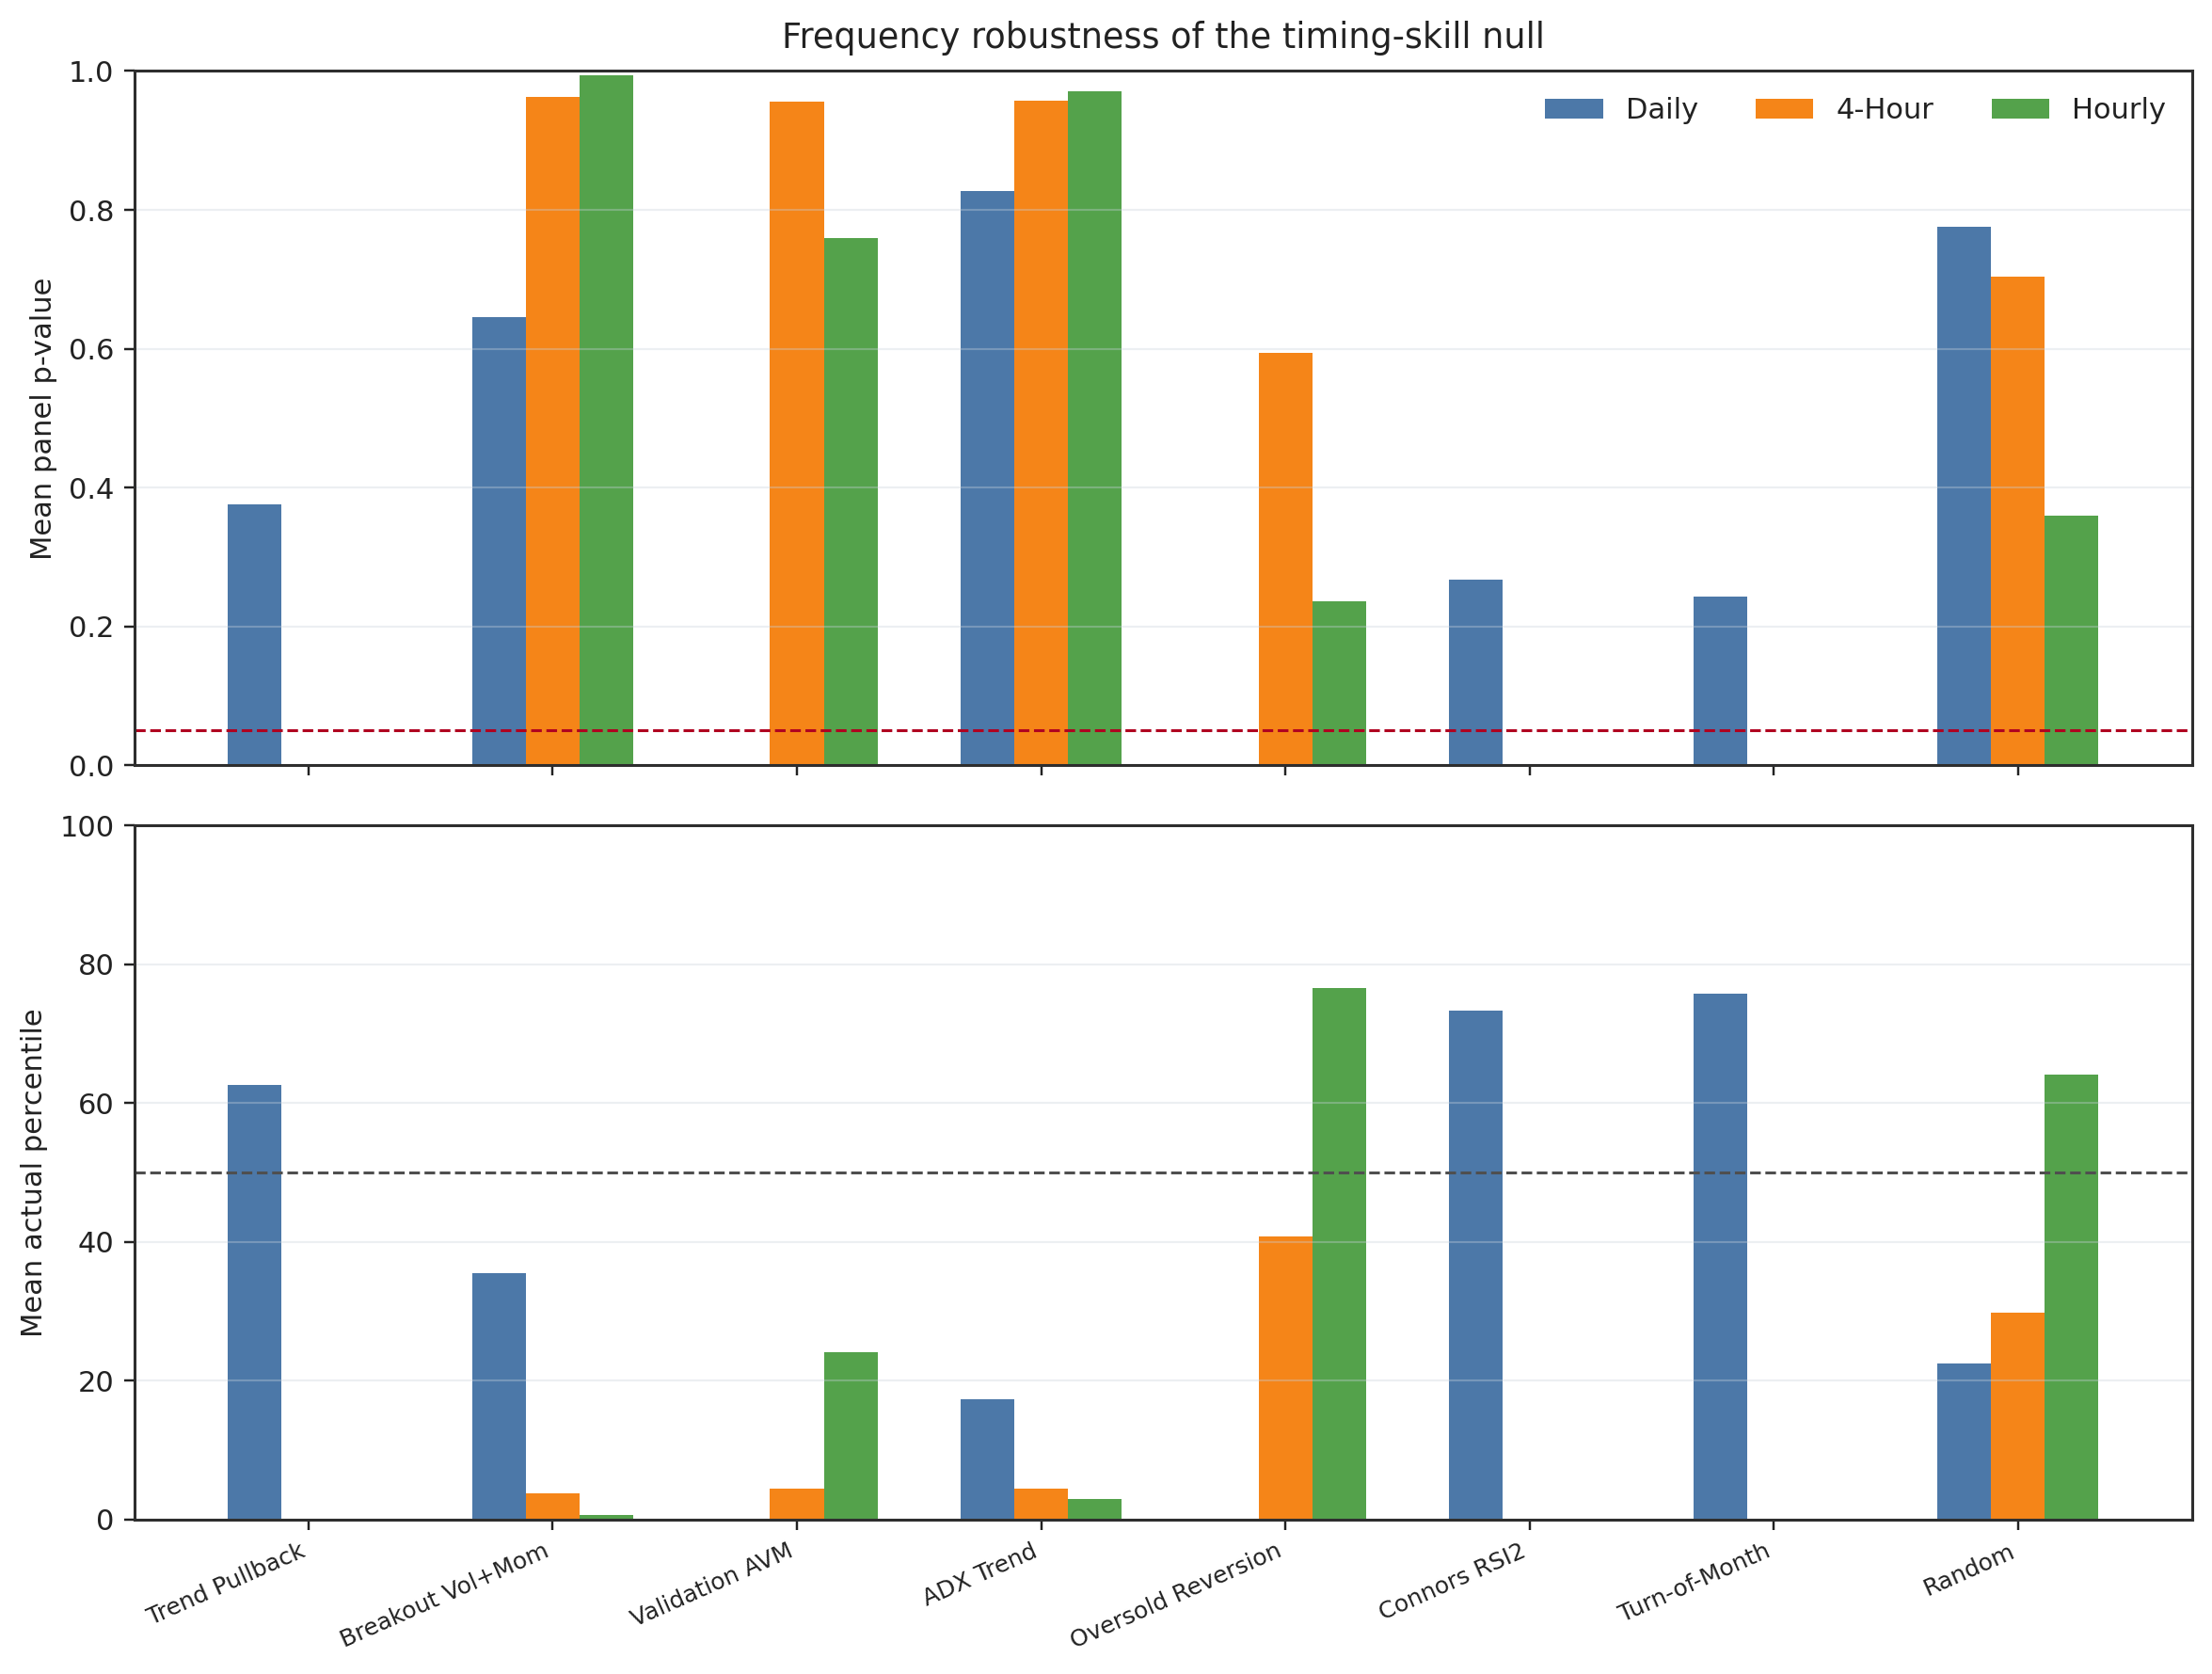
\includegraphics[width=0.95\textwidth]{frequency_robustness_pvalue_percentile.png}
\caption{Frequency-robustness check across recent daily, 4-hour, and hourly panels. The top panel reports mean panel $p$-value by strategy and interval; the bottom panel reports mean actual percentile.}
\label{fig:frequency_robustness}
\end{figure}

The frequency check does not overturn the main result; still, with at most five retained panels per interval it is underpowered to do so (Figure~\ref{fig:frequency_robustness}). The 4-hour panel is uniformly weak, with no retained strategy averaging above the null median and a best mean $p$-value of 0.593. The hourly panel contains one favorable mean-reversion result: Oversold Reversion averages percentile 76.5 with mean $p=0.236$ and one significant panel among five retained panels. That evidence is positive but not decisive, especially because the Random baseline also looks favorable on this small hourly slice. We therefore keep the interpretation modest: shortening the bar interval does not reveal broad, stable entry-placement skill, though the sparse hourly panel motivates a larger seed-robust intraday study.

\subsection{Anatomy of the above-median strategies}

The four above-median (not significant) strategies, namely Squeeze Breakout ($p=0.053$, percentile $94.7$), ADX Trend ($p=0.141$, percentile $85.9$), Connors RSI2 ($p=0.143$, percentile $85.7$), and Breakout Vol+Mom ($p=0.176$, percentile $82.4$), share one trait: each embeds an explicit regime or volatility filter (volatility compression, confirmed trend strength, short-term oversold extremes, or participation-plus-momentum confirmation) that concentrates entries in structurally favorable environments and so acts as an implicit timing mechanism. None crosses $p\le0.05$, but each modestly beats random placement, and their percentile placements are stable across robustness seeds (standard deviations of $0.3$ to $0.5$ points), so the classifications are not artifacts of a single simulation draw. By contrast, the strategies classified as random or luck use broader entry conditions (Turn-of-Month a calendar rule, Donchian Reentry a breakout-only filter) that dilute any conditional advantage. Specificity in entry conditions, not complexity, is what separates the above-median rules from those indistinguishable from random placement. None, however, reaches significance.

\subsection{Per-strategy Monte Carlo distribution summaries}

Each Monte Carlo distribution figure reports the realized outcome, the null median, null 5th and 95th percentiles, and the derived $p$-value and percentile. Table \ref{tab:mc} compiles these verified caption values in one place.

\clearpage
\begin{table}[p]
\centering
\caption{Monte Carlo distribution summaries per strategy (all values taken from the strategy-specific distribution captions, $M=5{,}000$).}
\label{tab:mc}
{\small
\renewcommand{\arraystretch}{1.15}
\setlength{\tabcolsep}{6pt}
\begin{adjustbox}{max width=\textwidth}
\begin{tabular}{@{}lrrrrrr@{}}
\toprule
Strategy & Actual & Null median & Null 5th & Null 95th & $p$-value & Percentile \\
\midrule
Trend Pullback      & 0.0832 & 0.4013 & -0.0611 & 1.0725 & 0.8700 & 13.0 \\
Breakout Vol+Mom    & 0.2967 & 0.1285 & -0.1215 & 0.4419 & 0.1758 & 82.4 \\
Mean Rev Vol Filter & -0.0097 & 0.0199 & -0.0897 & 0.1436 & 0.662\phantom{0} & 33.8 \\
Validation AVM      & 0.2187 & 0.1429 & -0.1285 & 0.4919 & 0.3447 & 65.5 \\
ADX Trend           & 0.8032 & 0.3705 & -0.0928 & 1.0660 & 0.1414 & 85.9 \\
Oversold Reversion  & 0.0822 & 0.0464 & -0.1007 & 0.2126 & 0.3409 & 65.9 \\
Squeeze Breakout    & 0.0649 & 0.0107 & -0.0483 & 0.0655 & 0.0534 & 94.7 \\
Connors RSI2        & 0.1184 & 0.0216 & -0.1112 & 0.1736 & 0.1428 & 85.7 \\
Donchian Reentry    & 0.0713 & 0.1462 & -0.1328 & 0.5173 & 0.6469 & 35.3 \\
Turn-of-Month       & 0.3229 & 0.1553 & -0.1498 & 0.5794 & 0.2336 & 76.7 \\
Random              & 0.6011 & 0.9381 & \phantom{-}0.1276 & 2.3314 & 0.7103 & 29.0 \\
\bottomrule
\end{tabular}
\end{adjustbox}
}
\par\vspace{0.75em}
\begin{minipage}{0.95\textwidth}
\centering
\footnotesize\emph{Notes.} ``Null'' values summarize the structure-preserving Monte Carlo distribution for each strategy as displayed in the per-strategy distribution figures. Each caption reports transaction cost $c=0.000470$.
\end{minipage}
\end{table}
\clearpage

Table \ref{tab:mc} makes the inference problem concrete. For several strategies, the realized outcome sits well inside the null distribution, despite positive profit. Trend Pullback illustrates this. Its return is 0.0832, while the null median is 0.4013 and the p-value is 0.8700. A profitability-only verdict would call this strategy successful. Yet under the structure-preserving null it underperforms random timing: its realized entries are \emph{worse} than what chance would typically produce.

\subsection{Regime-preserving schedule measure and exact small-$N$ enumeration}

\paragraph{Regime-preserving measure.} The context-matched measure of the main paper
matches each randomized entry to the realized entry's trailing-volatility quantile. As
a robustness check of the four context-matched rejections, we evaluate a second
volatility-state measure that discretizes the same state differently: the
\emph{regime-preserving} measure restricts each randomized entry to bars carrying the
same forward-safe volatility-regime label (calm, neutral, or stressed) as the bar the trade
actually occupied. The regime labels are the expanding-quantile volatility regimes of
Section~\ref{supp:implementation} (shifted by one bar, hence measurable at
entry); the construction reuses the candidate-pool sampler, substituting the regime
label for the volatility quantile. The sampler draws each entry from its trade's
same-regime pool restricted to the feasible window, and falls back to a regime-agnostic
uniform draw on the rare window that contains no same-regime bar. Run on the eleven-rule GC=F panel
(\texttt{MONTE\_CARLO\_REGIME\_MATCHING=1 MEASURE\_LABEL=regime\_preserving} on
\texttt{Code/schedule\_measure\_sensitivity.py}; output
\texttt{Data\_Clean/GC=F\_sensitivity\_regime\_preserving.csv}), it rejects exactly the
four strategies the context-matched measure rejects (Breakout Vol+Mom $p=0.037$, ADX
Trend $p=0.012$, Squeeze Breakout $p=0.032$, Connors RSI2 $p<0.001$) and no others,
while the neutral gap-permutation and leading-gap measures reject none. The same harness
reproduces the gap-permutation and context-matched columns of the main paper exactly,
confirming the regime variant does not perturb the canonical path. Both the regime tercile and the context-matched quintile are discretizations of
trailing realized volatility, so their agreement does not isolate placement from the
volatility-state channel; what it rules out is a binning- or construction-specific
matched-pool artifact, since a coarse forward-safe tercile and a finer in-sample quintile
flag exactly the same four. The evidence therefore identifies a volatility-regime-conditional
placement effect that the neutral, regime-agnostic measure conditions away. Measure-invariant
skill, rejection under every measure including the neutral ones, still fails.

\paragraph{Exact enumeration at $N=4$.} For the Squeeze Breakout strategy ($N=4$) the
gap-permutation orbit is small enough to enumerate exactly. The last exit is invariant
to the gap permutation, so every leading gap in $\{0,\dots,470\}$ is feasible, and the
orbit is exactly $3!\times(470{+}1)=2{,}826$ schedules. Its internal gaps
($834,4094,637$) are distinct, so all $2{,}826$ schedules yield distinct statistic
values: the attainable grid is fine, not atomic. Computing the cumulative return of
every schedule from the committed open-price path under the deterministic cost
convention ($c=0.000470$) gives an exact one-sided tail probability of $0.057$ for the
realized schedule, short of the $5\%$ threshold and consistent with the canonical Monte Carlo
$p=0.053$, which uses the stochastic-fill execution model; a $20{,}000$-draw Monte Carlo run
under the same deterministic-cost model returns $0.060$, confirming the exact value (\texttt{Code/squeeze\_exact\_enumeration.py}; output
\texttt{Data\_Clean/GC=F\_squeeze\_exact\_enumeration.csv}). The exact enumeration
therefore confirms the non-rejection and shows that the near-threshold reading at $N=4$
reflects weak identification of the placement margin (only $3!=6$ internal-gap
arrangements carry spacing information, while the leading gap relocates the whole
template in calendar time), not a coarse or atomic $p$-grid.

\section{Market regime analysis}

The regime figures are descriptive diagnostics, not separate hypothesis tests. They summarize trade-level performance using a trade-level return ratio defined as mean return divided by standard deviation, a Sharpe-like ratio per trade rather than an annualized Sharpe. The regime heatmap (Figure~\ref{fig:regime_heatmap}) reports values and trade counts per regime, suppressing regime cells with fewer than five trades, because a cell built on a handful of trades carries no reliable signal. The heatmap reports 11 suppressed cells. Many regime cells remain small even after suppression; for this reason we use the regime section to generate hypotheses about conditional behavior rather than to establish regime-specific timing skill.

Table \ref{tab:regimes} reproduces the verified regime values shown in the heatmap. We mark cells not shown in the heatmap as suppressed.

\begin{table}[htbp]
\centering
\caption{Regime-level trade performance (trade-level return ratio) taken from the regime heatmap. Values are shown as ratio with trade count in parentheses.}
\label{tab:regimes}
\small
\renewcommand{\arraystretch}{1.1}
\begin{tabular}{lccc}
\toprule
Strategy & Calm & Neutral & Stressed \\
\midrule
Trend Pullback      & 0.02 (n=10) & 0.13 (n=25) & 0.03 (n=42) \\
Breakout Vol+Mom    & 0.22 (n=14) & 0.14 (n=24) & 0.29 (n=8) \\
Mean Rev Vol Filter & -0.26 (n=10) & suppressed & suppressed \\
Validation AVM      & 0.34 (n=13) & 0.15 (n=22) & suppressed \\
ADX Trend           & 0.16 (n=50) & 0.27 (n=60) & suppressed \\
Oversold Reversion  & 0.29 (n=18) & 0.18 (n=12) & suppressed \\
Squeeze Breakout    & suppressed & suppressed & suppressed \\
Connors RSI2        & 0.17 (n=18) & 0.30 (n=23) & suppressed \\
Donchian Reentry    & 0.02 (n=28) & 0.08 (n=32) & suppressed \\
Turn-of-Month       & 0.10 (n=80) & 0.21 (n=61) & suppressed \\
Random              & 0.01 (n=76) & 0.11 (n=66) & 0.14 (n=73) \\
\bottomrule
\end{tabular}
\end{table}

Three regime patterns emerge, each with implications for the timing-skill interpretation.

First, several strategies show their strongest trade-level ratios in Neutral regimes. ADX Trend reaches 0.27 (n=60) in Neutral versus 0.16 (n=50) in Calm, and Connors RSI2 reaches 0.30 (n=23) in Neutral versus 0.17 (n=18) in Calm. This suggests that timing skill, to the extent it exists, concentrates in moderate-volatility environments where trends are identifiable but not disrupted by extreme price action. In other words, Neutral regimes offer a favorable signal-to-noise ratio: volatility is enough to generate meaningful moves but not so extreme as to overwhelm technical signals.

Second, Breakout Vol+Mom is the only strategy with strong Stressed-regime performance at 0.29 (n=8) in the regime heatmap (Figure~\ref{fig:regime_heatmap}); with only eight trades this cell is hypothesis-generating rather than confirmatory, and regime cells below roughly twenty trades should be read the same way. The result is consistent with the strategy's design, because its volume and momentum filters select Stressed-period entries where a genuine breakout occurs rather than a false signal. The suppression of most Stressed-regime cells across the panel (contributing to the 11 suppressed cells) shows that most strategies either avoid Stressed periods through explicit regime filters or generate too few trades in those periods to evaluate. This systematic avoidance is itself informative. The regime filters embedded in many strategies function as implicit timing mechanisms that concentrate trades in calmer environments; this explains part of their weak timing advantage.

Third, the Random baseline serves as a control. Its trade-level ratios are low but positive across all three regimes: 0.01 (n=76) in Calm, 0.11 (n=66) in Neutral, and 0.14 (n=73) in Stressed, with roughly even trade counts. This confirms that long-biased random exposure generates positive per-trade returns in all environments when the underlying asset appreciates. Profitability alone therefore does not distinguish skill from drift. Rule-based strategies show \emph{higher} ratios in specific regimes while the random baseline is uniformly mediocre, which suggests that the timing advantage is regime-conditional rather than universal.

\section{Robustness across Monte Carlo seeds}

Seed robustness matters because a single simulation run produces a single null distribution, and the resulting $p$-value and percentile are themselves random variables that depend on the pseudo-random seed. This means that if a strategy's classification changes across seeds, the single-run verdict is unreliable. We address this by evaluating each strategy under 100 independent outer runs, each with 5{,}000 simulations per run and transaction cost 0.000470, which produces a distribution of skill metrics rather than a single point estimate.

\subsection{RCSI stability}

The RCSI robustness chart reports mean $\pm$ SD across seeds. Deterministic strategies show small dispersions. Trend Pullback reports $-0.361 \pm 0.005$ and ADX Trend reports $0.387 \pm 0.005$. These intervals confirm that, for deterministic strategies, the null distribution is stable across seeds and the RCSI is a reliable point estimate of timing quality. Random, by contrast, shows high variability at $-0.103 \pm 0.523$, which is consistent with the strategy being stochastic under outer-run variation; both the realized trade sequence and the null distribution change across seeds, so the instability compounds.

\subsection{Percentile stability}

The percentile robustness chart (Figure~\ref{fig:pct_robust}) reports mean $\pm$ SD percentile across seeds. Squeeze Breakout reports $94.3 \pm 0.3$, ADX Trend reports $86.2 \pm 0.4$, and Breakout Vol+Mom reports $82.7 \pm 0.5$. Random reports $48.3 \pm 25.6$, consistent with extreme instability across seeds.

These robustness results support three claims. First, the above-median classifications for Squeeze Breakout, ADX Trend, Connors RSI2, and Breakout Vol+Mom are stable across seeds. Their percentile placements vary by less than one percentage point across 100 seeds, which shows that their relative positions in the null distribution are robust features of the data rather than artifacts of a particular simulation draw. Second, instability in the Random baseline's percentile ($\pm 25.6$) shows that stochastic strategies require seed-level robustness analysis; a single-run percentile of 29.0 would have been 75 or 5 under a different seed, so any single-run verdict is meaningless. Third, the contrast between the stable above-median strategies and the unstable random baseline shows that their percentile positions are stable features of the data rather than simulation noise. We are careful to read this as a statement about stability, not significance: none of these strategies reaches $p\le0.05$.

\section{Figures}
\label{sec:figures-gallery}

The figures in this section are regenerated directly from the canonical trade logs and the structure-preserving null by \texttt{Code/regenerate\_gallery.py}, which reproduces the published Monte Carlo distribution statistics exactly (the script aborts on any material mismatch). They are not transcribed raster outputs.

\begin{figure}[htbp]
\centering
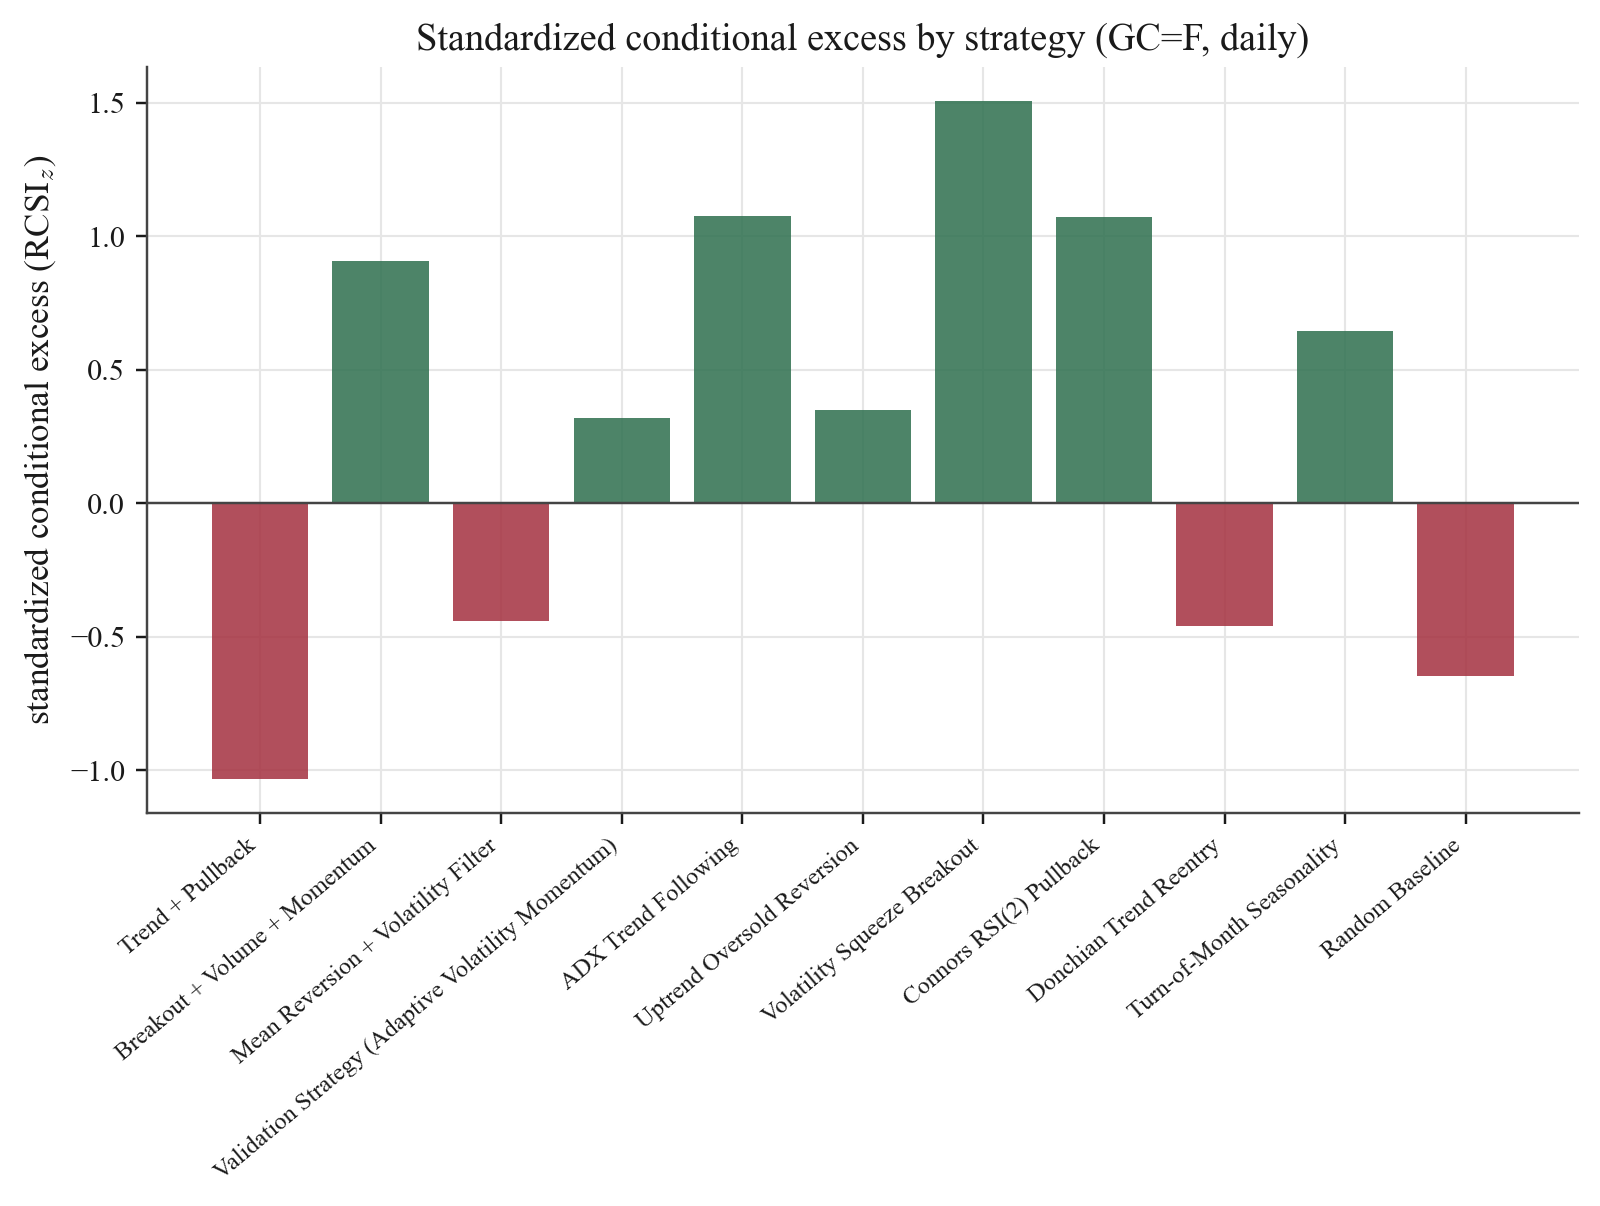
\includegraphics[width=0.85\textwidth]{rcsi_by_strategy.png}
\caption{GC=F. Conditional excess return (RCSI) by strategy (daily). The plot defines positive RCSI as performance above the strategy-specific Monte Carlo median, and uses RCSI along with $p$-value and percentile for classification.}
\label{fig:rcsi_by_strategy}
\end{figure}


\begin{figure}[htbp]
\centering
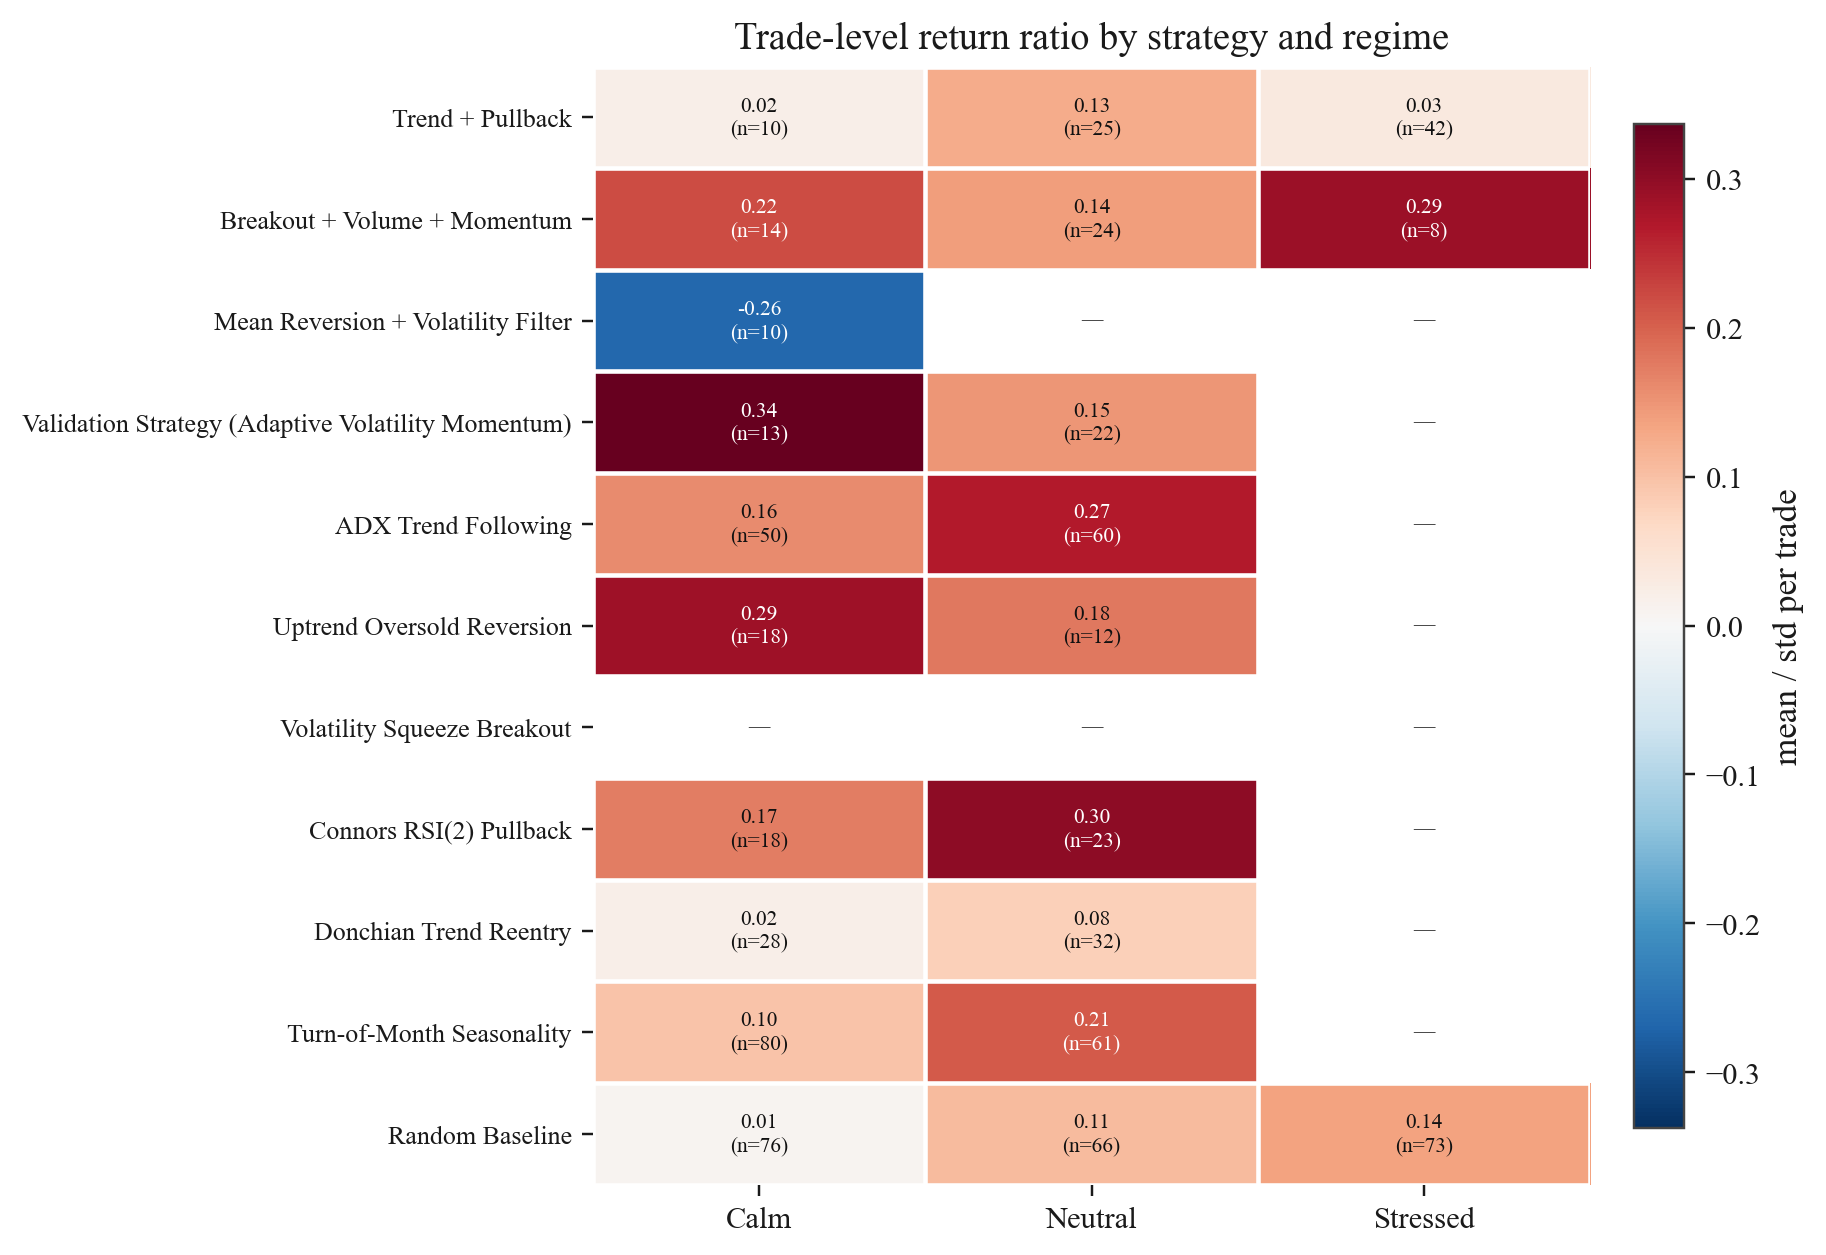
\includegraphics[width=0.66\textwidth]{regime_heatmap.png}
\caption{GC=F. Strategy performance across market regimes (daily). Cells show the trade-level return ratio and trade count: e.g., Breakout Vol+Mom is 0.22 (n=14) in Calm, 0.14 (n=24) in Neutral, and 0.29 (n=8) in Stressed. The figure reports ``Suppressed cells: 11'' for regimes with fewer than five trades.}
\label{fig:regime_heatmap}
\end{figure}

\begin{figure}[htbp]
\centering
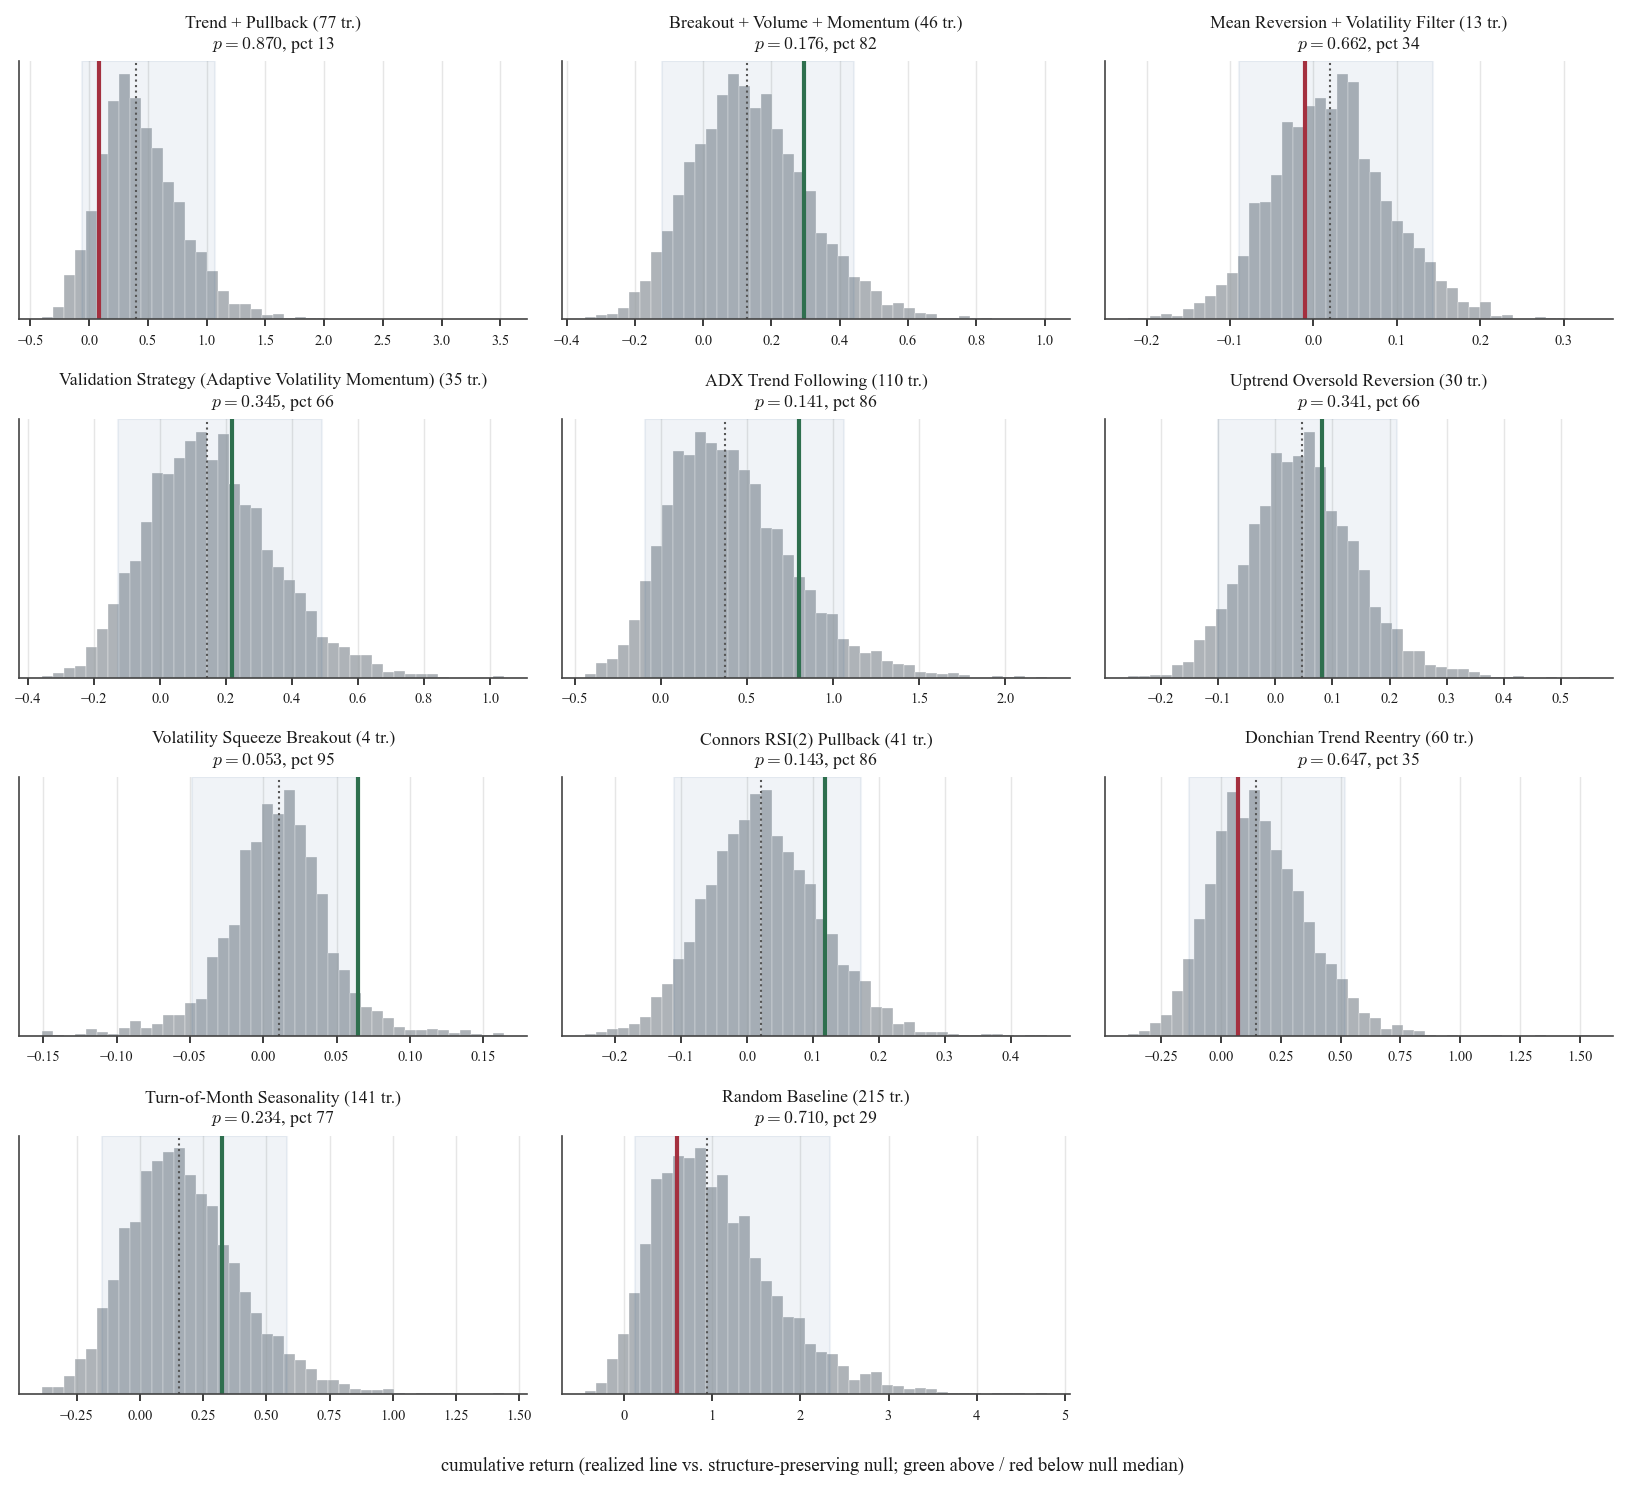
\includegraphics[width=\textwidth]{mc_panel.png}
\caption{GC=F. Structure-preserving Monte Carlo null distributions for all eleven strategies (daily, $M=5{,}000$, transaction cost $0.000470$). In each panel the grey histogram is the null of cumulative returns under randomized placement, the dotted line its median, the shaded band its $5$--$95$th percentiles, and the vertical line the realized return: green when above the null median, red when below. The realized line sits inside the bulk of the null for almost every strategy; only Squeeze Breakout (top of its tail, but $N_s=4$) approaches the upper edge. Exact per-strategy values appear in Table~\ref{tab:mc}.}
\label{fig:mc_panel}
\end{figure}

\begin{figure}[htbp]
\centering
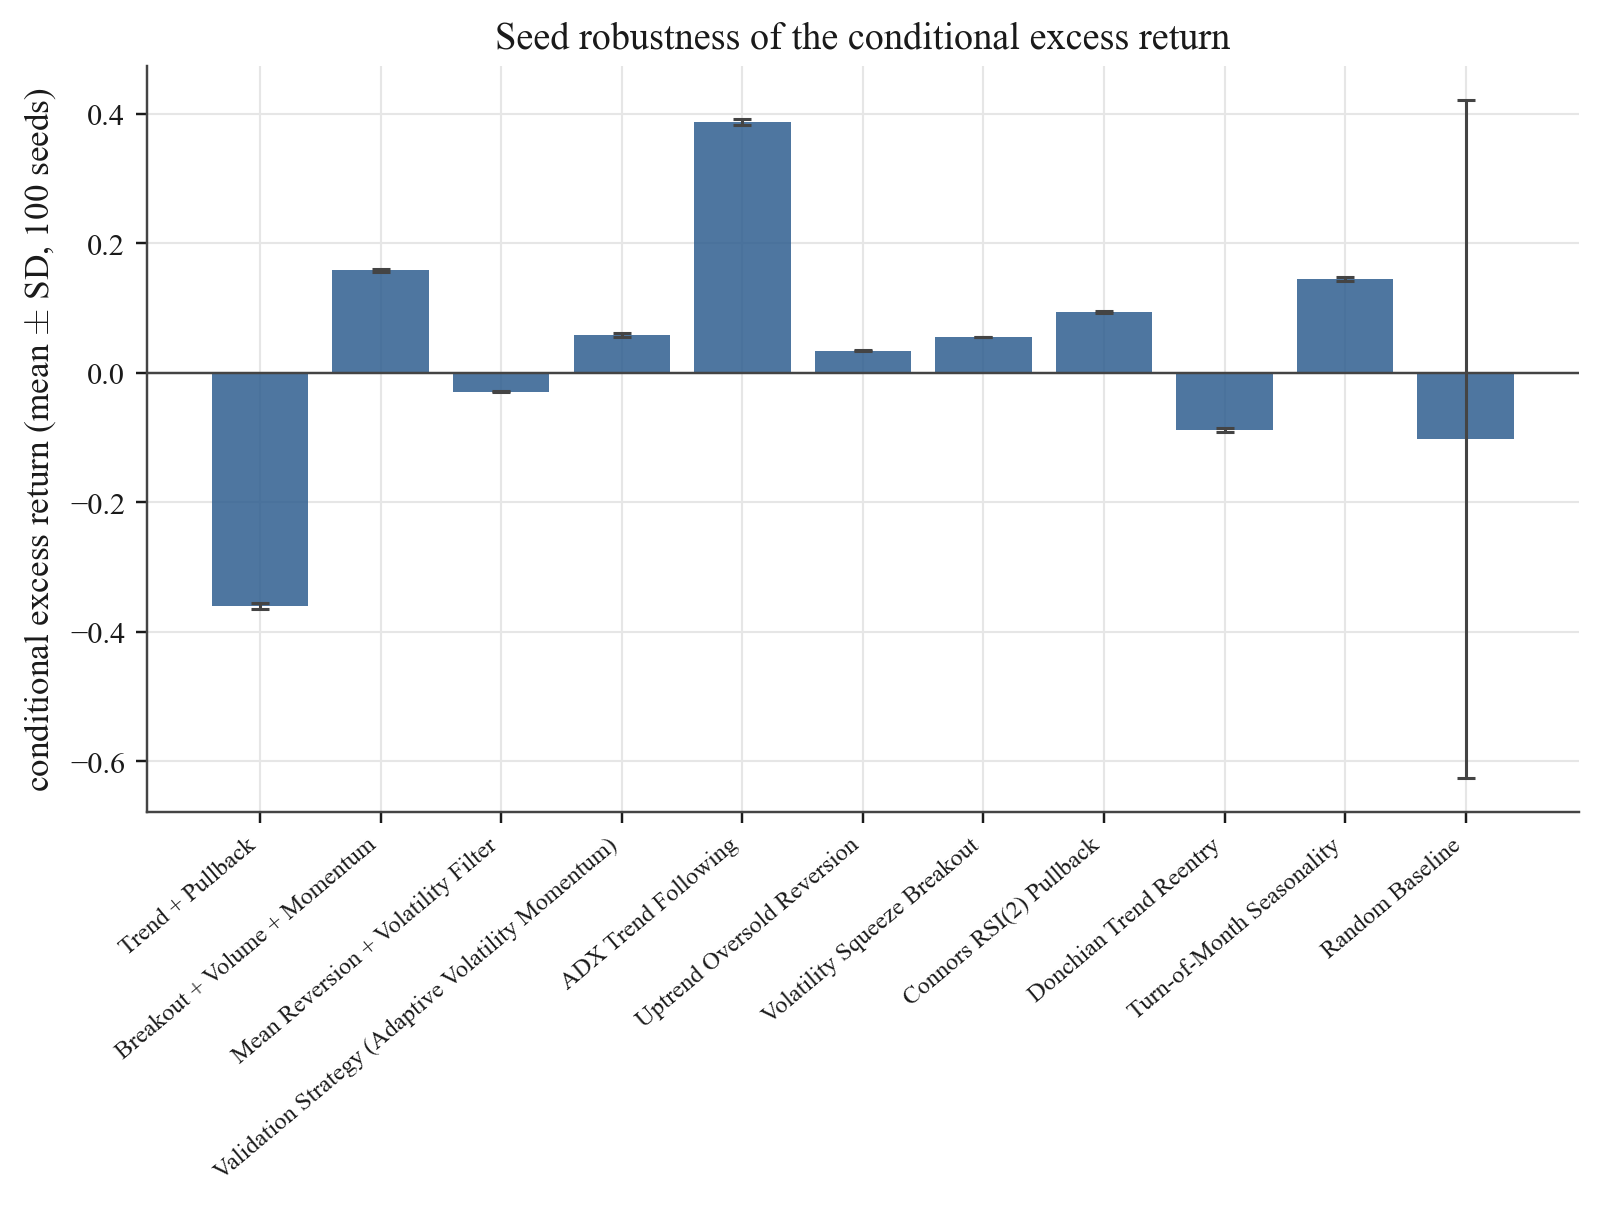
\includegraphics[width=0.85\textwidth]{rcsi_robustness.png}
\caption{GC=F. Monte Carlo robustness of RCSI across seeds (daily). The figure reports mean $\pm$ SD across outer runs, with outer runs = 100 and simulations per run = 5{,}000. Examples: Trend Pullback $-0.361\pm0.005$; ADX Trend $0.387\pm0.005$; Random $-0.103\pm0.523$. Transaction cost = 0.000470.}
\label{fig:rcsi_robust}
\end{figure}

\begin{figure}[htbp]
\centering
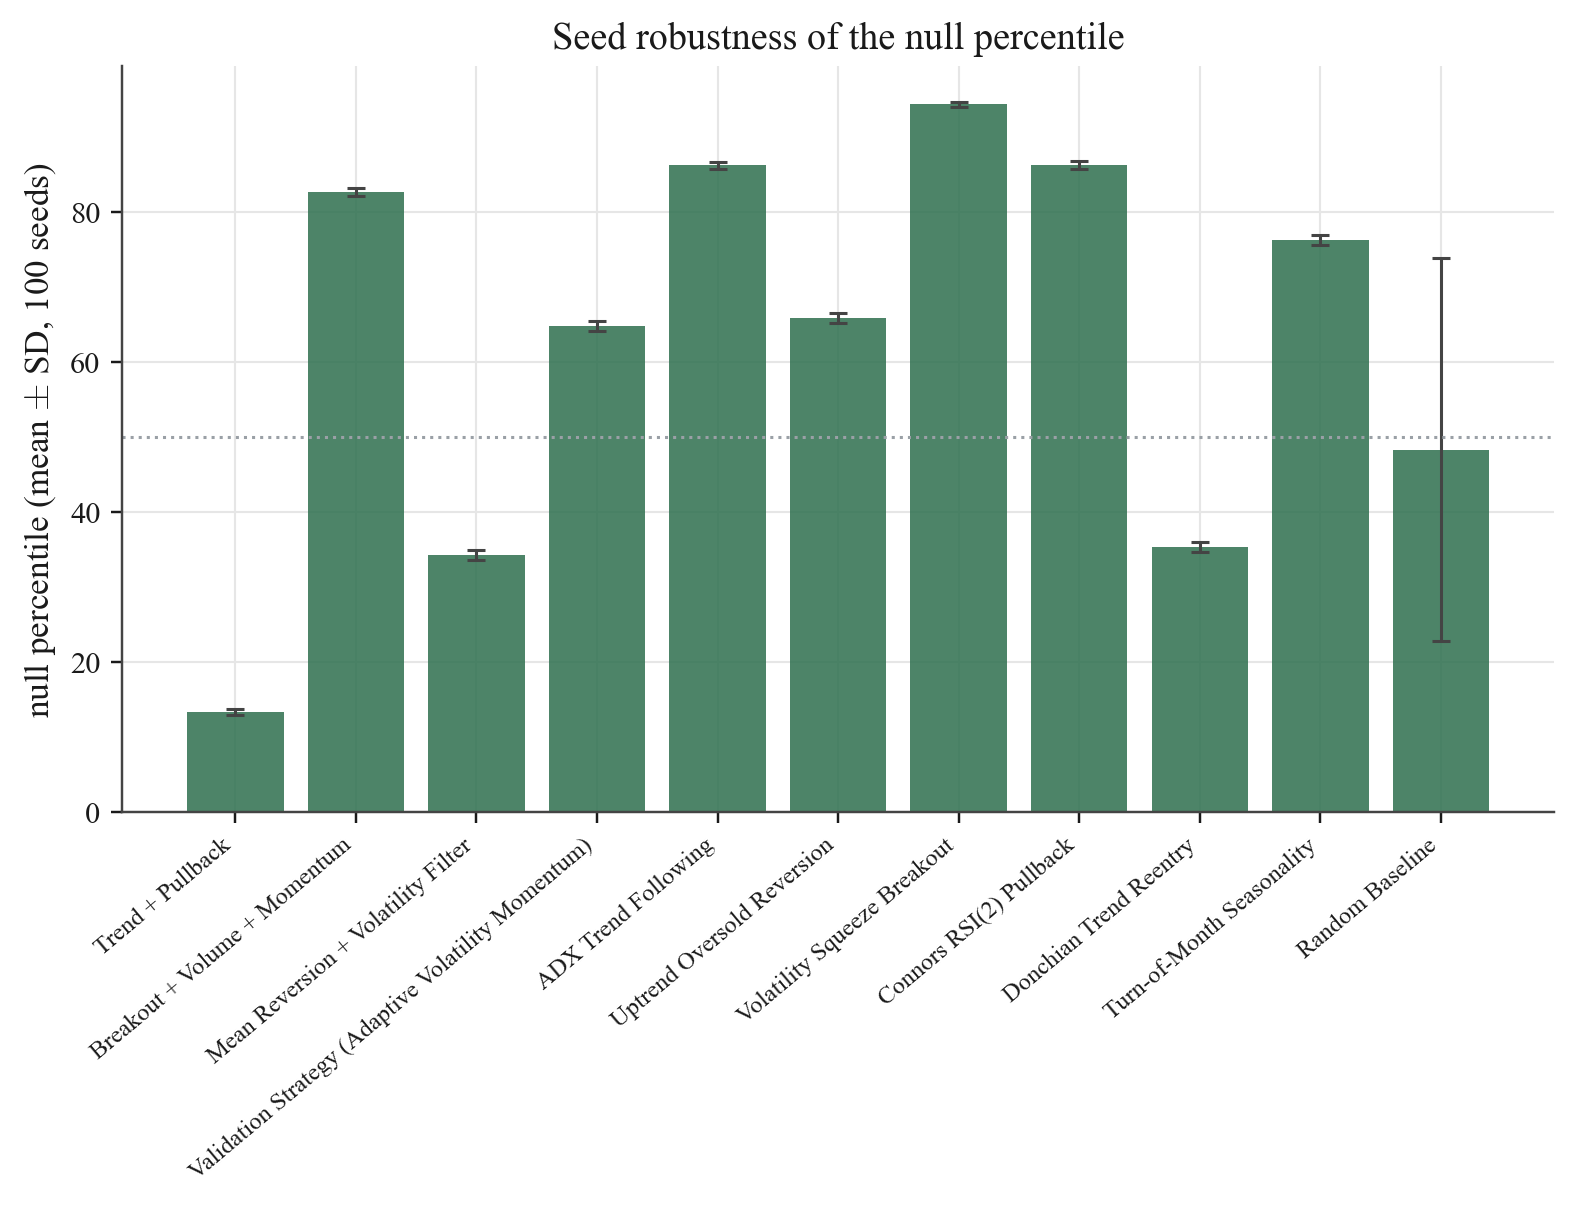
\includegraphics[width=0.85\textwidth]{percentile_robustness.png}
\caption{GC=F. Monte Carlo robustness of actual percentile across seeds (daily). Mean $\pm$ SD across outer runs. Examples: Squeeze Breakout $94.3\pm0.3$; ADX Trend $86.2\pm0.4$; Breakout Vol+Mom $82.7\pm0.5$; Random $48.3\pm25.6$.}
\label{fig:pct_robust}
\end{figure}

\begin{figure}[htbp]
\centering
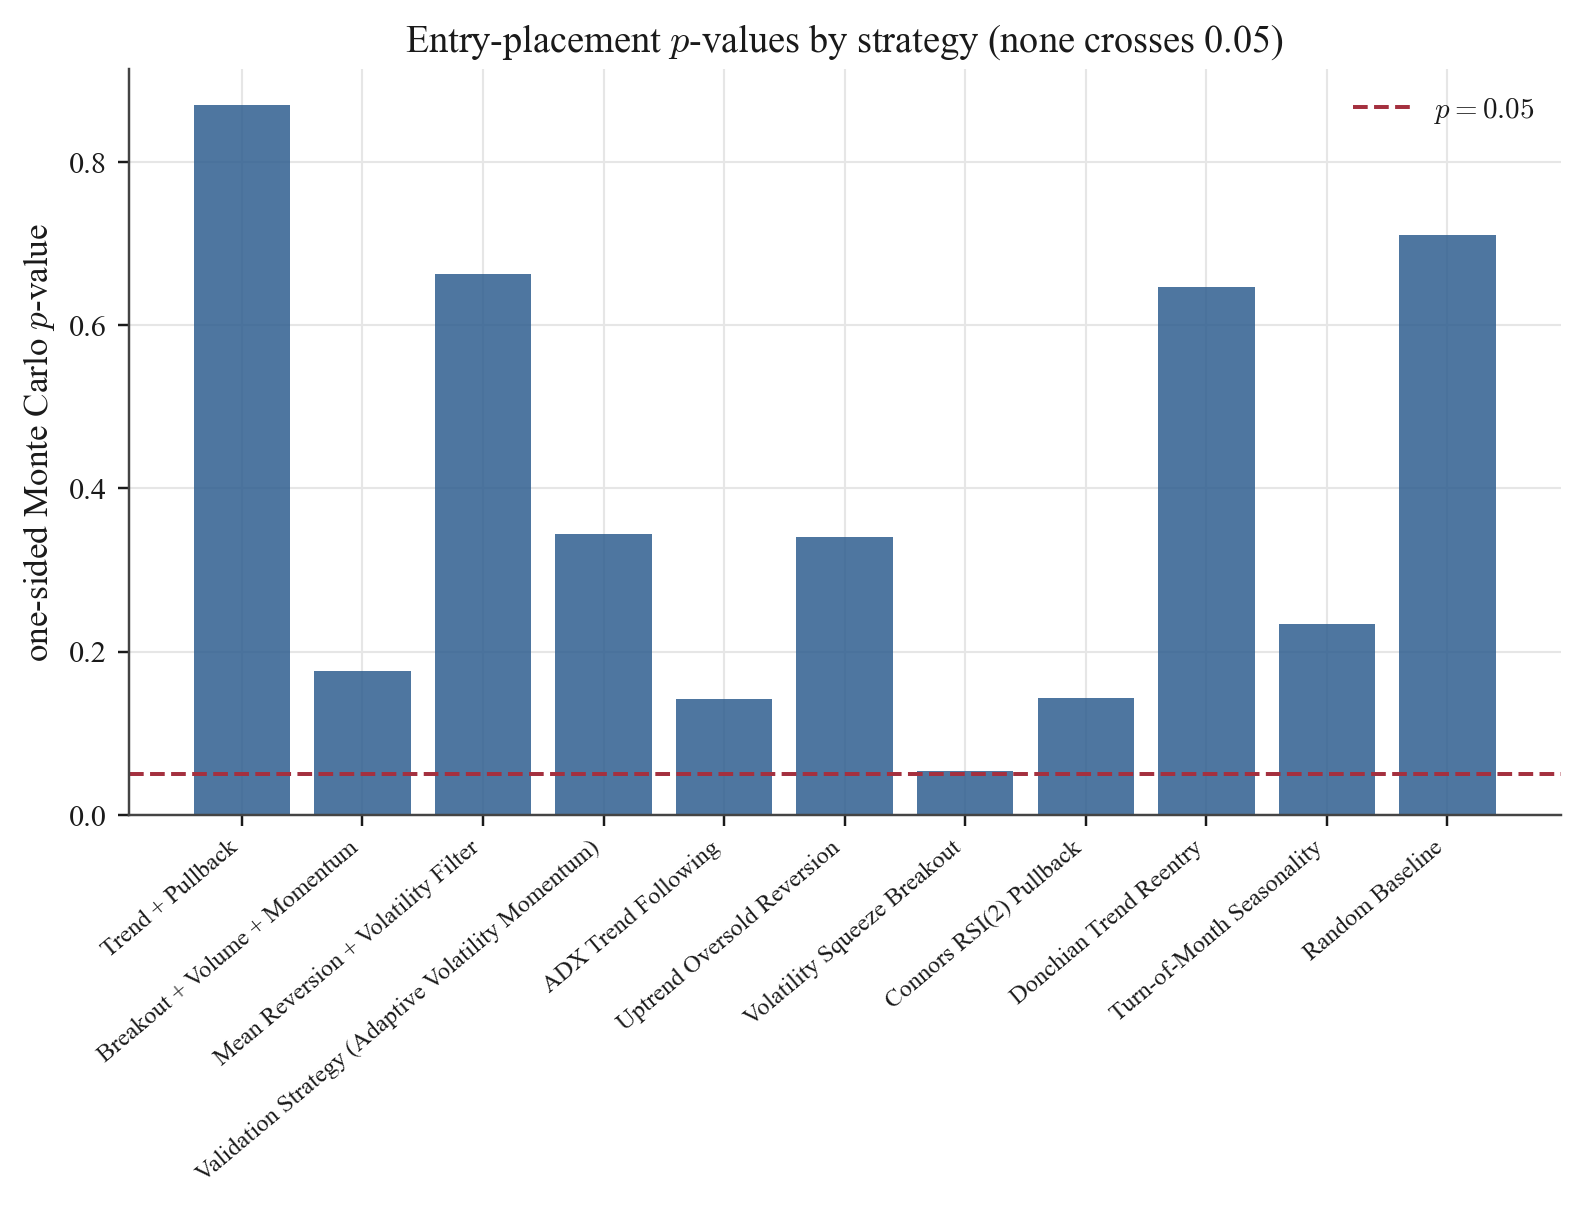
\includegraphics[width=0.85\textwidth]{pvalue_by_strategy.png}
\caption{GC=F. Monte Carlo p-value by strategy (daily). The dashed reference line marks the conventional threshold $p=0.05$. None of the plotted p-values crosses this threshold.}
\label{fig:pval_by_strategy}
\end{figure}

\begin{figure}[htbp]
\centering
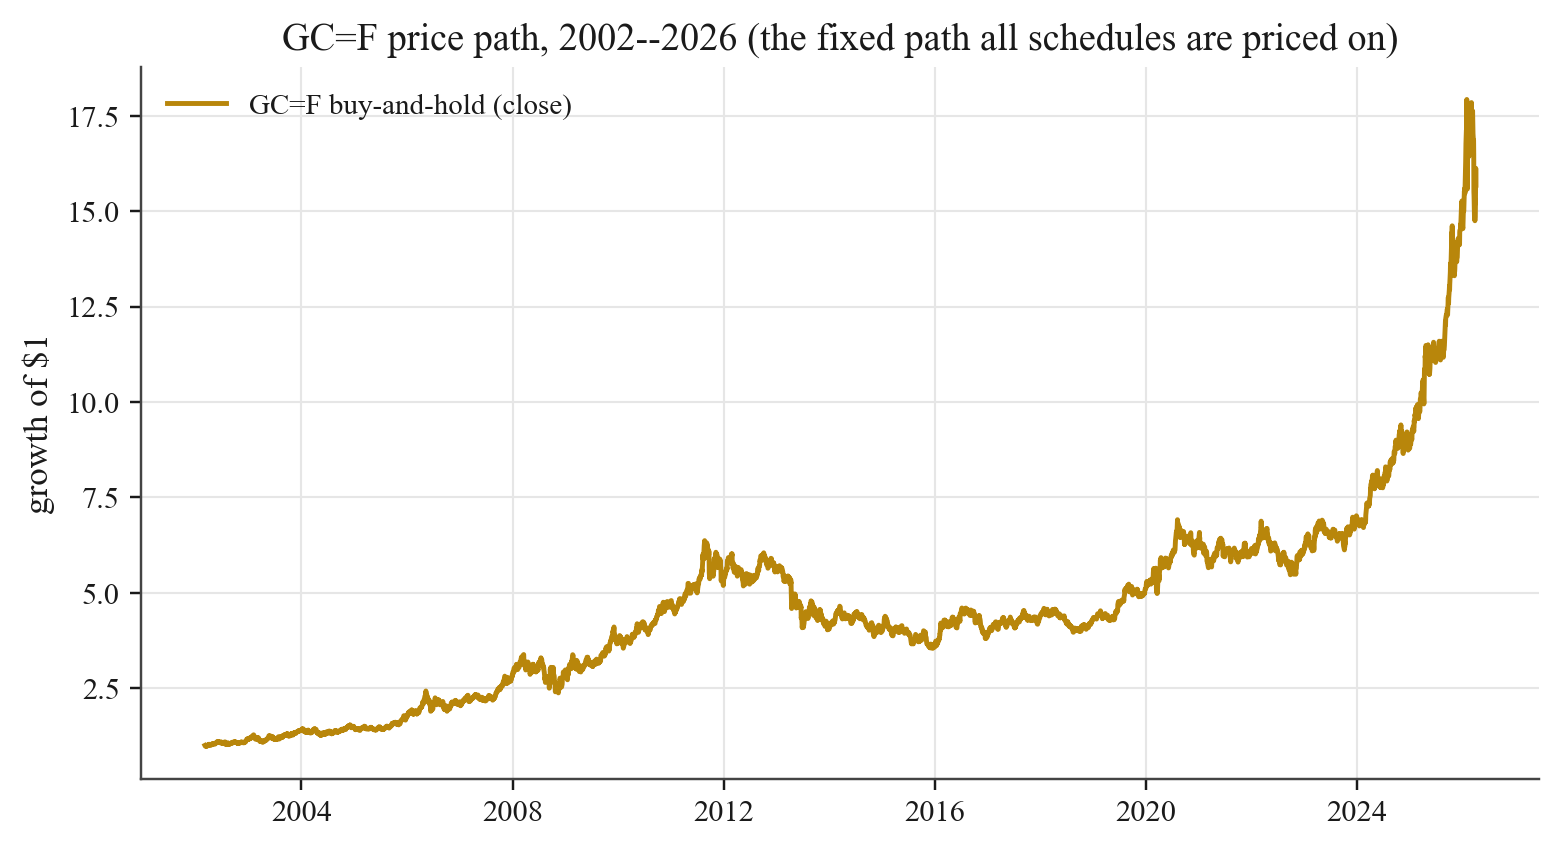
\includegraphics[width=0.85\textwidth]{equity_curve.png}
\caption{GC=F. Equity curves by strategy and benchmark (daily). Caption values list final cumulative returns: Trend Pullback 0.083; Breakout Vol+Mom 0.297; Mean Rev Vol Filter -0.010; Validation AVM 0.219; ADX Trend 0.803; Oversold Reversion 0.082; Squeeze Breakout 0.065; Connors RSI2 0.118; Donchian Reentry 0.071; Turn-of-Month 0.323; Random 0.601; Buy \& Hold 14.670. Sample window: 2002-03-04 00:00 to 2026-04-02 00:00.}
\label{fig:equity_curves}
\end{figure}

\section{Reproducibility}
\label{supp:repro}

\textbf{Code and data availability.} All code and the derived data required to reproduce every table and figure in this paper are publicly available at \url{https://github.com/ampatel355/FORTUNAFRAMEWORK} and permanently archived at \url{https://doi.org/10.5281/zenodo.20724999}. The repository contains the structure-preserving null implementation, the analysis scripts referenced in this appendix, the regime-labeled price series and realized trade logs, and a \texttt{README} mapping each table and figure to its exact reproduction command. Runs are deterministic under the seed protocol described below.

\subsection{Figure-based data sources}

The GC=F empirical panel (cumulative returns, trade counts, Monte Carlo $p$-values, percentiles, $\mathrm{RCSI}_z$, regime ratios, and seed robustness in Table~\ref{tab:main}) is reproduced directly from the canonical trade logs and the structure-preserving null by \texttt{Code/regenerate\_gallery.py} (Monte Carlo distributions, conditional excess, $p$-values, and regime ratios) and the robustness summary (seed-level dispersion); the gallery figures of the previous section are produced by the same script. The script verifies its regenerated statistics against the reported values and aborts on any material mismatch, so figures and text cannot silently diverge.

\subsection{Computed analyses and exact commands}

The computed analyses below are generated directly from the accompanying code rather than transcribed, so they reproduce exactly. The synthetic validation (Table~\ref{tab:synthetic_validation}, Figures~\ref{fig:synthetic_calibration} and~\ref{fig:synthetic_power}) is produced, from base seed $9100$, by
\begin{verbatim}
SYNTHETIC_REPLICATIONS=1500 SYNTHETIC_POWER_REPLICATIONS=400 \
SYNTHETIC_SIMULATIONS=2000 \
  ./.venv/bin/python Code/synthetic_timing_experiments.py
\end{verbatim}
which writes \texttt{Data\_Clean/synthetic\_null\_validation\_summary.csv}. The schedule-measure sensitivity (Table~\ref{tab:schedule_sensitivity}) re-evaluates the fixed GC=F trade logs under each measure with $M=5{,}000$ simulations and the seed-$42$ spawn protocol:
\begin{verbatim}
MEASURE_LABEL=baseline \
  ./.venv/bin/python Code/schedule_measure_sensitivity.py
MONTE_CARLO_MIN_LEADING_INDEX=200 \
  MEASURE_LABEL=leading_gap_200 \
  ./.venv/bin/python Code/schedule_measure_sensitivity.py
MONTE_CARLO_CONTEXT_MATCHING=1 \
  MEASURE_LABEL=context_matched \
  ./.venv/bin/python Code/schedule_measure_sensitivity.py
\end{verbatim}
The baseline column reproduces Table~\ref{tab:main} exactly, confirming the harness matches the canonical pipeline; results are written to \texttt{Data\_Clean/\allowbreak GC=F\_sensitivity\_*.csv}.

The real-data positive control (Table~\ref{tab:positive_control}, Figures~\ref{fig:pc_curve} and~\ref{fig:pc_hist}) injects a tunable fraction of well-timed entries into a strategy on the GC=F open-price series and scores it against the structure-preserving null with execution-cost simulation disabled, over $100$ seeds at $M=5{,}000$:
\begin{verbatim}
  PC_SEEDS=100 ./.venv/bin/python Code/positive_control_power.py
\end{verbatim}
which writes \texttt{Data\_Clean/\allowbreak GC=F\_positive\_control\_power\_summary.csv}; setting \texttt{MONTE\_CARLO\_SIMULATE\_EXECUTION\_COSTS=1} reruns it with stochastic execution costs enabled and writes the \texttt{\_costson\_} variant. The cross-asset multiplicity panel (Table~\ref{tab:cross_asset_multiplicity}, Figure~\ref{fig:cross_asset}) aggregates the saved \texttt{Data\_Clean/*\_full\_comparison.csv} run outputs and applies Benjamini--Hochberg and Bonferroni control across all $322$ tests:
\begin{verbatim}
  ./.venv/bin/python Code/cross_asset_multiplicity.py
\end{verbatim}
which writes \texttt{Data\_Clean/cross\_asset\_panel\_summary.csv}. The realistic-signal detection results (Table~\ref{tab:signal_mechanisms}, Figure~\ref{fig:signal_curve}) and the regenerated GC=F figure gallery (Section~\ref{sec:figures-gallery}, Table~\ref{tab:main}) are produced by
\begin{verbatim}
  ./.venv/bin/python Code/positive_control_signals.py
  ./.venv/bin/python Code/regenerate_gallery.py
\end{verbatim}
The latter recomputes the eleven Monte Carlo distributions, the conditional excess, the $p$-values, and the regime ratios from the canonical trade logs and verifies them against the reported values before writing any figure. The head-to-head competitor comparison (Table~\ref{tab:competitor}, Figure~\ref{fig:competitor}) runs all four tests on the five known-truth worlds with a fixed, world-offset seed protocol ($400$ replications, $M=2{,}000$ structure-preserving draws, $B=999$ bootstrap resamples, block length $20$):
\begin{verbatim}
CC_REPLICATIONS=400 CC_BOOT=999 CC_SIMULATIONS=2000 \
  PYTHONHASHSEED=0 ./.venv/bin/python \
  Code/competitor_comparison.py
\end{verbatim}
which writes \texttt{Data\_Clean/competitor\_comparison.csv}.

\subsection{Statement on empirical integrity}

The GC=F empirical panel is reproduced from the canonical trade logs and the structure-preserving null by the commands in this appendix, which verify their regenerated statistics against the reported values and abort on any material mismatch; this means every value in the computed analyses is the direct output of those commands on the accompanying data. Where a quantity was produced by neither source, we state it qualitatively and do not invent a numeric estimate; this is a deliberate, conservative choice.

\bibliographystyle{elsarticle-num}

\begin{thebibliography}{99}

\bibitem{fama1970}
E. F. Fama, Efficient capital markets: A review of theory and empirical work,
\emph{The Journal of Finance} 25(2) (1970) 383--417.

\bibitem{lo2004}
A. W. Lo, The adaptive markets hypothesis: Market efficiency from an evolutionary perspective,
\emph{The Journal of Portfolio Management} 30(5) (2004) 15--29.

\bibitem{white2000}
H. White, A reality check for data snooping,
\emph{Econometrica} 68(5) (2000) 1097--1126.

\bibitem{hansen2005}
P. R. Hansen, A test for superior predictive ability,
\emph{Journal of Business \& Economic Statistics} 23(4) (2005) 365--380.

\bibitem{sullivan1999}
R. Sullivan, A. Timmermann, H. White, Data-snooping, technical trading rule performance, and the bootstrap,
\emph{The Journal of Finance} 54(5) (1999) 1647--1691.

\bibitem{bailey2017}
D. H. Bailey, J. M. Borwein, M. L\'opez de Prado, Q. J. Zhu,
The probability of backtest overfitting,
\emph{Journal of Computational Finance} 20(4) (2017) 39--69.

\bibitem{moskowitz2012}
T. J. Moskowitz, Y. H. Ooi, L. H. Pedersen, Time series momentum,
\emph{Journal of Financial Economics} 104(2) (2012) 228--250.

\bibitem{politisromano1994}
D. N. Politis, J. P. Romano, The stationary bootstrap,
\emph{Journal of the American Statistical Association} 89(428) (1994) 1303--1313.

\bibitem{benjaminihochberg1995}
Y. Benjamini, Y. Hochberg, Controlling the false discovery rate: A practical and powerful approach to multiple testing,
\emph{Journal of the Royal Statistical Society, Series B} 57(1) (1995) 289--300.

\bibitem{romanowolf2005}
J. P. Romano, M. Wolf, Stepwise multiple testing as formalized data snooping,
\emph{Econometrica} 73(4) (2005) 1237--1282.

\bibitem{harveyliuzhu2016}
C. R. Harvey, Y. Liu, H. Zhu, $\ldots$ and the cross-section of expected returns,
\emph{Review of Financial Studies} 29(1) (2016) 5--68.

\bibitem{lopezdeprado2018}
M. L\'opez de Prado, \emph{Advances in Financial Machine Learning}, Wiley, 2018.

\bibitem{baileylopez2014}
D. H. Bailey, M. L\'opez de Prado, The deflated Sharpe ratio: Correcting for selection bias, backtest overfitting, and non-normality,
\emph{Journal of Portfolio Management} 40(5) (2014) 94--107.

\bibitem{Fisher1935}
R. A. Fisher, \emph{The Design of Experiments}, Oliver \& Boyd, Edinburgh, 1935.

\bibitem{LehmannRomano2005}
E. L. Lehmann, J. P. Romano, \emph{Testing Statistical Hypotheses}, 3rd Edition, Springer, New York, 2005.

\bibitem{Candes2018}
E. Cand\`es, Y. Fan, L. Janson, J. Lv, Panning for gold: `model-X' knockoffs for high dimensional controlled variable selection,
\emph{Journal of the Royal Statistical Society: Series B} 80(3) (2018) 551--577.

\bibitem{Ernst2004}
M. D. Ernst, Permutation methods: A basis for exact inference,
\emph{Statistical Science} 19(4) (2004) 676--685.

\bibitem{Aldous1985}
D. J. Aldous, Exchangeability and related topics, in: \emph{\'Ecole d'\'Et\'e de Probabilit\'es de Saint-Flour XIII---1983}, Lecture Notes in Mathematics, vol.~1117, Springer, Berlin, 1985, pp.~1--198.

\bibitem{Dwass1957}
M. Dwass, Modified randomization tests for nonparametric hypotheses,
\emph{The Annals of Mathematical Statistics} 28(1) (1957) 181--187.

\bibitem{Hope1968}
A. C. A. Hope, A simplified Monte Carlo significance test procedure,
\emph{Journal of the Royal Statistical Society: Series B} 30(3) (1968) 582--598.

\bibitem{HemerikGoeman2018}
J. Hemerik, J. Goeman, Exact testing with random permutations,
\emph{TEST} 27(4) (2018) 811--825.

\bibitem{PhipsonSmyth2010}
B. Phipson, G. K. Smyth, Permutation $p$-values should never be zero: Calculating exact $p$-values when permutations are randomly drawn,
\emph{Statistical Applications in Genetics and Molecular Biology} 9(1) (2010) Article 39.

\bibitem{BesagClifford1989}
J. Besag, P. Clifford, Generalized Monte Carlo significance tests,
\emph{Biometrika} 76(4) (1989) 633--642.

\bibitem{PesarinSalmaso2010}
F. Pesarin, L. Salmaso, \emph{Permutation Tests for Complex Data: Theory, Applications and Software}, John Wiley \& Sons, Chichester, 2010.

\bibitem{FithianSunTaylor2014}
W. Fithian, D. Sun, J. Taylor, Optimal inference after model selection,
arXiv:1410.2597 (2014).

\bibitem{LeeSunSunTaylor2016}
J. D. Lee, D. L. Sun, Y. Sun, J. E. Taylor, Exact post-selection inference, with application to the lasso,
\emph{The Annals of Statistics} 44(3) (2016) 907--927.

\bibitem{BerkBrownBujaZhangZhao2013}
R. Berk, L. Brown, A. Buja, K. Zhang, L. Zhao, Valid post-selection inference,
\emph{The Annals of Statistics} 41(2) (2013) 802--837.

\bibitem{Kunsch1989}
H. R. K\"unsch, The jackknife and the bootstrap for general stationary observations,
\emph{The Annals of Statistics} 17(3) (1989) 1217--1241.

\bibitem{Storey2002}
J. D. Storey, A direct approach to false discovery rates,
\emph{Journal of the Royal Statistical Society: Series B} 64(3) (2002) 479--498.

\bibitem{BenjaminiYekutieli2001}
Y. Benjamini, D. Yekutieli, The control of the false discovery rate in multiple testing under dependency,
\emph{The Annals of Statistics} 29(4) (2001) 1165--1188.

\end{thebibliography}

\end{document}
